% !TeX root = main.tex

\documentclass[12pt, a4paper, oneside]{book}

% --- Pakete ---
\usepackage[utf8]{inputenc}
\usepackage[T1]{fontenc}
\usepackage{lmodern}
\usepackage[ngerman]{babel}
\usepackage{pdfpages}
\usepackage{microtype}
\usepackage[title, titletoc]{appendix}
\usepackage{acronym}
% 1. Macht die gesamte erste Nennung kursiv
\renewcommand*{\acffont}[1]{\textit{#1}}

% 2. Hebt das Kursive für die Klammer und die Kurzform wieder auf
\renewcommand*{\acfsfont}[1]{\textup{#1}}

% Zitierstil (BibLaTeX mit Biber)
\usepackage[backend=biber, style=apa]{biblatex}
\addbibresource{literatur.bib} % Deine exportierte Datei

\begin{document}
\frontmatter
\begin{titlepage}
    \title{Konzeption und Evaluation eines Multi-Agenten-Systems zur automatisierten Migration von imperativer LO-VC Logik zu deklarativer AVC Syntax am Beispiel der msg systems ag }
    \author{Torben Dörrer}
\end{titlepage}
\maketitle
\tableofcontents
\newpage
% !TeX root = main.tex

\section*{Abkürzungsverzeichnis} % Sternchen verhindert eine Kapitelnummer
\addcontentsline{toc}{section}{Abkürzungsverzeichnis} % Fügt es zum Inhaltsverzeichnis hinzu

% Das längste Kürzel (z.B. [HTTPS]) in die eckigen Klammern setzen. 
% Das sorgt für einen sauberen, einheitlichen Abstand im Verzeichnis.

\begin{acronym}[HTTPS]
    \acro{KMAT}{konfigurierbare Materialstamm}
    \acro{Super BOM}{konfigurierbare Maximalstückliste}
    \acro{AVC}{Advanced Variant Configuration}
    \acro{LO-VC}{Logistics Variant Configuration}
    \acro{KI}{künstliche Intelligenz}
    \acro{ML}{Machine Learning}
    \acro{CSP}{Constraint Satisfaction Problem}
    \acro{LLMs}{Large Language Models}
    \acro{LLM}{Large Language Model}
    \acro{ICL}{In-Context Learning}
    \acro{MAS}{Multi-Agenten-Systems}
    \acro{DSR}{Design Science Research}
    \acro{POC}{Proof of Concept}
    \acro{FF}{Forschungsfragen}
    \acro{API}{Application Programming Interface}
    \acro{ERP}{Enterprise Resource Planning}
    \acro{PO}{Product Owner}
    \acro{JSON}{JavaScript Object Notation}
    \acro{SAT}{Boolean Satisfiability Problem}
    \acro{AST}{Abstract Syntax Tree}
    \acro{SQL}{Structured Query Language}
\end{acronym} 
\newpage

\mainmatter
% !TeX root = ../main.tex
\chapter{Einleitung}
\label{ch:einleitung}

\section{Motivation und Problemstellung}
\label{sec:motivation_und_problemstellung}

Im Zuge der digitalen Transformation und der Abkündigung älterer ERP-Generationen stehen produzierende Unternehmen weltweit vor 
der komplexen Herausforderung, ihre IT-Landschaften auf das moderne System SAP S/4HANA zu migrieren. Ein hochgradig kritischer 
Teilbereich dieser Transition betrifft die Variantenkonfiguration: Die historisch gewachsene, imperative Logik der klassischen 
\ac{LO-VC} muss in die moderne, deklarative Syntax der \ac{AVC} überführt werden. 

In der industriellen Praxis – insbesondere im Beratungsumfeld der \textit{msg systems ag} – zeigt sich, dass diese 
Syntax-Migration einen massiven zeitlichen und finanziellen Flaschenhals darstellt. Da direkte, maschinelle 1:1-Übersetzer 
aufgrund der grundlegenden Paradigmenwechsel zwischen imperativen und deklarativen Regelwerken fehlen, erfolgt die Überführung 
oftmals in manueller, extrem fehleranfälliger Fleißarbeit. Erste Versuche der Industrie, diesen Prozess durch moderne generative 
\ac{KI} zu automatisieren, blieben bislang hinter den Erwartungen zurück. Wie Voruntersuchungen zeigen, 
scheitern monolithische Single-Prompt-Ansätze (wie die einfache Abfrage über Werkzeuge wie ChatGPT) an der strukturellen 
Komplexität und den strikten Syntaxvorgaben der SAP-Constraint-Netzwerke. Das Sprachmodell verliert bei langen Logikketten den 
Kontext und neigt zu nicht-kompilierbaren Halluzinationen. 

Um diesen Flaschenhals informationstechnisch aufzulösen, rückt das Paradigma der \ac{MAS} in den Fokus der angewandten Informatik. 
Die Hypothese lautet, dass eine Aufteilung von Teilbereichen der komplexen Übersetzungsaufgabe in ein orchestriertes Kollektiv spezialisierter 
KI-Agenten die Code-Qualität und die Arbeitsgeschwindigkeit bei der Migration drastisch erhöhen kann, sofern die Ergebnisse der \ac{KI} 
von Entwicklern in einem iterativen, agentischen Workflow validiert und konsolidiert werden.

\section{Zielsetzung und Forschungsfragen}
\label{sec:zielsetzung_und_forschungsfragen}

Das primäre Ziel dieser Masterarbeit ist die theoriegeleitete Konzeption und praktische Implementierung einer 
Multi-Agenten-Architektur zur automatisierten Code-Migration von LO-VC nach AVC. In Kooperation mit der \textit{msg systems ag} 
soll nicht nur die theoretische Eignung von Agenten-Frameworks evaluiert, sondern ein lauffähiger, cloudbasierter Prototyp auf 
der \textit{SAP Business Technology Platform} (BTP) entwickelt und bewertet werden.

Um dieses Ziel zu erreichen, wird die Arbeit von folgender Hauptforschungsfrage geleitet: 
\textbf{In welchem Umfang kann ein Multi-Agenten-System die Effizienz und Qualität bei der Migration von imperativer LO-VC-Logik 
zu deklarativer AVC-Syntax im Vergleich zum manuellen Vorgehen steigern?} 

Zur strukturierten Beantwortung dieser Hauptfrage werden vier dedizierte Unter-Forschungsfragen (FF) definiert:
\begin{itemize}
    \item \textbf{FF1 (Baseline):} Welche manuellen Prozessschritte sind bei der Migration zwingend erforderlich und wie hoch ist der zeitliche Aufwand pro Logik-Objekt?
    \item \textbf{FF2 (Werkzeug-Wahl):} Anhand welcher technischen und konzeptionellen Kriterien lässt sich das optimale Multi-Agenten-Framework (z.\,B. CrewAI vs. AutoGen vs. LangChain) für das Einsatzumfeld der automatisierten Code-Migration identifizieren und rechtfertigen?
    \item \textbf{FF3 (Architektur):} An welchen Stellen der Migration bietet sich der Einsatz eines \ac{MAS} an und wie lässt sich der herausgearbeitete Scope systematisch in spezialisierte agentische Rollen überführen?
    \item \textbf{FF4 (Impact):} Welche Einsparung (in Bearbeitungszeit) und welche Qualitätsrate (Syntax-Korrektheit) erzielt der agentische Ansatz im Vergleich zur manuellen Baseline?
\end{itemize}

\section{Methodisches Vorgehen und Forschungsdesign}
\label{sec:methodisches_vorgehen}

Um eine valide, praxistaugliche und wissenschaftlich fundierte Multi-Agenten-Architektur für die Migration von LO-VC- nach 
AVC-Code zu konzipieren, folgt diese Arbeit dem Paradigma des \ac{DSR} nach 
\textcite{hevnerDesignScienceInformation2004}. Ziel dieses gestaltungsorientierten Forschungsansatzes ist die Konstruktion und 
Evaluation eines innovativen, zweckmäßigen IT-Artefakts -- in diesem Fall des Modells und der nachfolgenden Instanziierung einer 
Multi-Agenten-System-Architektur --, um ein komplexes, unstrukturiertes Problem (\textit{Wicked Problem}) in einem realen 
technologischen Umfeld nachhaltig zu lösen. 

Entsprechend dem IS-Forschungsmethoden-Framework von \textcite{hevnerDesignScienceInformation2004} gliedert sich das 
Forschungsdesign dieser Arbeit in zwei komplementäre Kernphasen, welche die Balance zwischen praktischer Relevanz 
(\textit{Relevance}) und methodischer Strenge (\textit{Rigor}) sichern:

\begin{enumerate}
    \item \textbf{Explorative Phase zur Problem- und Scope-Definition (Umfeld \& Relevanz):} 
    Den Ausgangspunkt bildet die präzise Erfassung des Problemraums und des \textit{Business Needs} innerhalb des organisationalen 
    und technologischen Umfelds (\textit{Environment}). Hierzu wird eine explorative Fallstudie nach den Richtlinien von 
    \textcite{runesonGuidelinesConductingReporting2009} vorgeschaltet. Um Verzerrungen zu minimieren und den konkreten 
    funktionalen Scope des \ac{MAS} empirisch abzugrenzen, erfolgt eine Datentriangulation aus drei Quellen:
    \begin{itemize}
        \item \textit{Archivdokumentenanalyse:} Systematische Untersuchung bestehender SAP-Dokumentationen, Syntaxvorgaben und 
        Altsystemstrukturen zur Definition der technologischen Rahmenbedingungen.
        \item \textit{Qualitative Experteninterviews:} Erhebung von implizitem Praxiswissen (\textit{Tacit Knowledge}) von 
        Domänenexperten bezüglich manueller Migrationsaufwände (Baseline) sowie realer Fallstricke beim Einsatz generativer KI.
        \item \textit{Selbstversuch:} Durchführung einer eigenen, manuellen Beispielmigration zur Identifikation inhärenter 
        syntaktischer Transformationsbarrieren im LO-VC-Code.
    \end{itemize}
    Die Synthese dieser Erkenntnisse fundiert den Problemraum wissenschaftlich und führt direkt zur Ableitung einer ersten 
    fundierten Version 1 (V1) der Systemarchitektur.

    \item \textbf{Iterativer DSR-Gestaltungs- und Evaluationszyklus (Konstruktion \& Strenge):}
    Aufbauend auf der Architekturversion V1 setzt der eigentliche Kernprozess des Design Science Research ein. Im Sinne des von 
    \textcite{hevnerDesignScienceInformation2004} beschriebenen \textit{Generate/Test Cycle} (Suchprozess) wird das Artefakt im 
    Zuge der softwaretechnischen Umsetzung schrittweise und iterativ weiterentwickelt (V1 zu V2 bis zur finalen Architektur). 
    Jede Iteration greift dabei auf theoretische Grundlagen aus der Wissensbasis (\textit{Knowledge Base}) zurück -- wie etwa 
    etablierte Architekturmuster für Multi-Agenten-Systeme sowie Prinzipien des Compilerbaus --, um die methodische Strenge 
    (\textit{Rigor}) zu gewährleisten. Abschließend wird das fertige Artefakt einer rigorosen Evaluation 
    (z.\,B. durch funktionales Testing mit realitätsnahen Migrationsszenarien) unterzogen, um dessen Nützlichkeit 
    (\textit{Utility}) empirisch nachzuweisen.
\end{enumerate}

Durch diese methodische Verknüpfung wird sichergestellt, dass die vorgeschlagene MAS-Architektur nicht nur auf strengen 
wissenschaftlichen Methoden beruht, sondern auch einen messbaren, praktischen Beitrag für die automatisierte Code-Transformation 
in der industriellen SAP-Praxis leistet.

\section{Abgrenzung der Arbeit}
\label{sec:abgrenzung}

% TODO: Scope definieren. Hier wird später im Detail aufgeschlüsselt, welche spezifischen LO-VC Elemente (z.B. Constraints, Preconditions, Selection Conditions) der Prototyp transformieren kann und welche Sonderfälle oder komplexe Prozeduren (Procedures) bewusst aus dem Scope dieser Arbeit exkludiert werden.

\section{Aufbau der Arbeit}
\label{sec:aufbau_der_arbeit}

Die vorliegende Arbeit gliedert sich in sechs aufeinander aufbauende Kapitel. Nach der Einleitung in \textbf{Kapitel 1} schafft \textbf{Kapitel 2} das theoretische Fundament, indem es die Domäne der SAP-Variantenkonfiguration erläutert und die Paradigmen von Multi-Agenten-Systemen nach aktuellem Forschungsstand analysiert. In \textbf{Kapitel 3} erfolgt die Auswertung der Experteninterviews zur Festlegung der manuellen Baseline und der funktionalen Anforderungen. \textbf{Kapitel 4} widmet sich dem praktischen Selbstversuch, in dem die Auswahl des Frameworks, die Rollenspezifikation und die Integration in die SAP BTP dokumentiert werden. \textbf{Kapitel 5} umfasst die Evaluation des entwickelten Prototyps anhand der Forschungsfragen, um die messbaren Mehrwerte und Limitierungen gegenüber der Baseline darzustellen. Die Arbeit schließt in \textbf{Kapitel 6} mit einem Resümee und einem Ausblick auf zukünftige Forschungspotenziale.
% !TeX root = ../main.tex
\chapter{Theoretische Grundlagen}
\label{ch:theory}
\section{Domänenspezifische Grundlagen: SAP Variantenkonfiguration}
\subsection{Einführung in die logische Architektur der Variantenkonfiguration}

In der modernen Fertigungsindustrie erfordert die Abbildung kundenindividueller Produkte hochflexible 
Systemstrukturen. Die grundlegende informationstechnische Idee der Variantenkonfiguration besteht darin, ein 
Produkt durch eine Vielzahl möglicher Ausprägungen zu definieren, welche durch ein iteratives Regelwerk logisch 
miteinander verknüpft sind, um komplexe Geschäftsprozesse strukturiert abzubilden. Da die Ausmultiplikation aller 
möglichen Kombinationsmöglichkeiten die Anzahl der Varianten schnell in die Millionen oder in extremen Fällen der 
Anlagenfertigung bis in den Bereich von Quadrillionen ($10^{24}$) treiben kann, ist die Anlage diskreter Stammdaten 
für jede einzelne Ausprägung in der Praxis unmöglich (zitat). 

Als systemtechnische Antwort auf diese kombinatorische Explosion fungiert im SAP-System der sogenannte 
\textit{konfigurierbare Materialstamm} (KMAT). 
Dieser dient als universaler Platzhalter, unter dem die gesamte Variantenvielfalt eines Produkts 
informationstechnisch zusammengefasst wird (zitat). 
Um diese Vielfalt in einer sogenannten Bewertungsoberfläche abzubilden, greift die SAP-Architektur auf 
drei zentrale Strukturkomponenten zurück (zitat):

\begin{itemize}
    \item \textbf{Merkmale (Characteristics):} Sie definieren die spezifischen Eigenschaften eines Produkts 
    (wie beispielsweise die Lackierung oder die Traglast eines Gabelstaplers).
    \item \textbf{Variantenklassen:} Diese dienen der logischen Bündelung der Merkmale und werden direkt dem 
    konfigurierbaren Materialstamm zugeordnet.
    \item \textbf{Konfigurationsprofil:} Dieses fungiert als übergeordnetes Steuerungselement, das die Stammdaten 
    zusammenhält und den Konfigurationsprozess maßgeblich regelt.
\end{itemize}

Ein zentrales Paradigma der SAP-Variantenkonfiguration zur Bewältigung dieser Komplexität ist das sogenannte 
Maximal-Prinzip. Anstatt ein Produkt aus einzelnen Modulen additiv zu einem 100\,\%-Modell zusammenzusetzen, 
basiert die Architektur auf einem subtraktiven 150\,\%-Modell. Hierfür wird eine 
\textit{konfigurierbare Maximalstückliste} (Super BOM) eingesetzt. Diese umfasst sämtliche Bauteile und 
Komponenten, die für jedwede theoretisch mögliche Variante des Produkts jemals benötigt werden könnten 
(zitat). Während des Konfigurationsprozesses können dieser Stückliste keine neuen 
Elemente hinzugefügt, sondern lediglich nicht benötigte Komponenten herausgefiltert werden.

Die logische Brücke zwischen der kaufmännischen Konfiguration und der technischen Fertigung bildet das 
\textit{Beziehungswissen} (Object Dependencies). Metaphorisch gesprochen übersetzt dieses Regelwerk das 
kundenseitige „Wünschen“ in der Bewertungsoberfläche in das fertigungsseitige „Erhalten“ in Form der ausgedünnten 
Stückliste (zitat). Konkret wird dies durch Steuerungsmechanismen wie 
\textit{Auswahlbedingungen} (Selection Conditions) realisiert. Wenn ein Kunde beispielsweise aus einem Angebot von 
sechs Motoren einen spezifischen Antrieb wählt, determinieren die Auswahlbedingungen des Beziehungswissens, 
dass die fünf nicht gewählten Motoren aus der finalen Fertigungsstückliste eliminiert werden 
(zitat). 

Die Zusammenhänge dieser fundamentalen Architekturkomponenten – vom konfigurierbaren Materialstamm über die 
Bewertungsoberfläche bis hin zur Maximalstückliste und dem steuernden Beziehungswissen – sind in Abbildung 
\ref{fig:variantenkonfig} schematisch zusammengefasst.

(Hier kommt die Grafik rein)

\subsection{Die klassische Variantenkonfiguration (LO-VC) im Kontext der Systemtransformation}
\label{sec:lovc_context}

Um die technologische Entwicklung der Variantenkonfiguration zu verstehen, ist zunächst eine Einordnung 
in die Evolution der SAP-Systemlandschaften erforderlich. Während das bisherige Kernprodukt 
\textit{SAP ERP} (oft auch als SAP R/3 bezeichnet) über Jahrzehnte den Standard darstellte, markiert 
\textit{SAP S/4HANA} eine fundamentale Neuausrichtung der Softwarearchitektur, insbesondere durch die 
Nutzung der In-Memory-Datenbanktechnologie \parencite[vgl.][S. 28]{blumohrAdvancedVariantConfiguration2023}. 
In diesem Zuge wurde für die Variantenkonfiguration ein neues technologisches Fundament geschaffen.

Der Begriff \textit{Logistics Variant Configuration} (LO-VC) dient heute primär als Retronym, um die 
klassische Art der Konfiguration von der neuen \textit{Advanced Variant Configuration} (AVC) abzugrenzen 
\parencite[vgl.][S. 32]{blumohrAdvancedVariantConfiguration2023}. Obwohl LO-VC in aktuellen S/4HANA-Installationen 
(On-Premise und Private Cloud) aus Gründen der Abwärtskompatibilität weiterhin verfügbar ist, gilt sie 
technologisch als veralteter Standard. 

Wie bereits in den Grundlagen erläutert, basiert LO-VC auf einem prozeduralen Paradigma, das historisch 
bedingt oft durch einen „Learning-by-Doing“-Ansatz in den Unternehmen gewachsen ist. Dies führte dazu, 
dass Modelle häufig unnötig komplex durch den Einsatz von Prozeduren und Aktionen anstatt 
leistungsfähigerer Constraints gestaltet wurden \parencite[vgl.][S. 58]{blumohrAdvancedVariantConfiguration2023}. Der Wechsel zu 
AVC wird in der Literatur daher nicht nur als technisches Upgrade, sondern als strategische Notwendigkeit 
beschrieben, die durch folgende Kernaspekte begründet wird:

\begin{itemize}
    \item \textbf{Rückkehr zum Standard und Vereinfachung:} AVC stellt den künftigen Standard dar. Die 
    Migration bietet Unternehmen die Chance, historisch gewachsene, schwer wartbare „Spaghetti-Logiken“ 
    zu dekonstruieren und durch eine moderne, leichter wiederverwendbare Modellierung zu ersetzen 
    \parencite[vgl.][S. 57\,f.]{blumohrAdvancedVariantConfiguration2023}.
    \item \textbf{Abbildung moderner Geschäftsmodelle:} Klassische LO-VC-Strukturen sind primär auf den 
    reinen Verkauf von Produkten (SD-Kontext) ausgelegt. Moderne Strategien wie das 
    \textit{Solution Bundling} (Kombination aus Produkt, Dienstleistung und Abonnements) lassen sich im 
    Standard nur über AVC und die damit verknüpften neuen Objektträger wie die \textit{Solution Quote} 
    abbilden \parencite[vgl.][S. 59]{blumohrAdvancedVariantConfiguration2023}.
    \item \textbf{Technologische Überlegenheit:} AVC nutzt mit \textit{Gecode} eine moderne 
    Constraint-Solving-Engine, die im Gegensatz zur sequenziellen LO-VC-Logik analytische Prinzipien 
    verfolgt und damit eine deutlich höhere Performance und Flexibilität bietet 
    \parencite[vgl.][S. 59]{blumohrAdvancedVariantConfiguration2023}.
    \item \textbf{Zukunftsfähigkeit (KI und Analytics):} Innovative Technologien wie 
    \textit{Artificial Intelligence} (AI) oder \textit{Machine Learning} (ML) sowie moderne 
    Auswertungsmethoden via \textit{CDS-Views} werden nativ für AVC entwickelt. Eine nachträgliche 
    Integration in die veraltete LO-VC-Architektur gleicht lediglich einer „Renovierung“, die nie den 
    Leistungsumfang einer Neuentwicklung erreichen kann \parencite[vgl.][S. 61]{blumohrAdvancedVariantConfiguration2023}.
    \item \textbf{Human-Resource-Aspekt:} Angesichts des Fachkräftemangels ist die Arbeit mit moderner 
    Softwarearchitektur ein entscheidender Faktor bei der Gewinnung von Talenten. Die Wartung einer über 
    25 Jahre alten Softwarelösung ist im Vergleich zur Vorreiterrolle in einer intelligenten 
    Fertigungsumgebung auf Basis aktueller Technologie weniger attraktiv für qualifizierten Nachwuchs 
    \parencite[vgl.][S. 60]{blumohrAdvancedVariantConfiguration2023}.
\end{itemize}

Zusammenfassend lässt sich festhalten, dass der Verbleib in der LO-VC-Welt zwar kurzfristig 
Transformationsaufwände vermeidet, langfristig jedoch das Risiko erhöht, den Anschluss an technologische 
Innovationen zu verlieren und den Aufwand für eine spätere Migration durch das wachsende technologische 
Delta exponentiell zu vergrößern \parencite[vgl.][S. 61]{blumohrAdvancedVariantConfiguration2023}.

\subsection{Die moderne Architektur (AVC) und das Constraint-Paradigma}
\label{sec:avc_constraint}

Die Antwort auf die konzeptionellen Schwächen und technischen Limitierungen der klassischen 
Variantenkonfiguration bildet die Einführung der \textit{Advanced Variant Configuration} (AVC) in SAP 
S/4HANA. Um den stetig wachsenden Anforderungen an Performance und Modellierungskomplexität 
(wie beispielsweise in den \textit{Make-to-Order}- oder \textit{Engineer-to-Order}-Szenarien) gerecht zu 
werden, vollzieht SAP mit AVC nicht nur ein syntaktisches Update, sondern einen fundamentalen 
informationstechnischen Paradigmenwechsel unter der Haube der Konfigurations-Engine 
\parencite[vgl.][S. 35]{blumohrAdvancedVariantConfiguration2023}.

Während das bisherige LO-VC-System, wie in Kapitel \ref{sec:lovc_context} beschrieben, auf einer 
iterativen, imperativen Abarbeitung von Befehlen und Prozeduren basierte, nutzt AVC einen grundlegend 
deklarativen Lösungsansatz. Das technologische Herzstück der AVC-Architektur bildet ein neu integrierter 
\textit{Constraint Solver} namens \textit{Gecode}, eine ursprünglich quelloffene Softwarebibliothek, 
die in Zusammenarbeit mit dem Fraunhofer-Institut ITWM tief in den SAP-Standard eingebettet und für 
komplexe Produktkonfigurationen erweitert wurde \parencite[vgl.][S. 35]{blumohrAdvancedVariantConfiguration2023}.

Der Einsatz dieser Engine überführt den Konfigurationsprozess mathematisch in ein sogenanntes 
\textit{Constraint Satisfaction Problem} (CSP). Bei einem CSP geht es aus informatischer Sicht nicht mehr 
darum, eine Liste von Instruktionen nacheinander abzuarbeiten, um einen Endzustand zu berechnen. 
Stattdessen wird das gesamte Modell als ein Netzwerk aus Variablen (den SAP-Merkmalen) und den 
zugehörigen Wertebereichen (den Domänen) definiert. Das Beziehungswissen wird in diesem Paradigma als 
harte Bedingungen (\textit{Constraints}) formuliert, die festlegen, welche Merkmalskombinationen 
zulässig sind und welche sich gegenseitig ausschließen. Ziel des CSP-Solvers ist es, eine gültige 
Belegung für alle Variablen zu finden, bei der kein einziger Constraint verletzt wird. 

Dieser deklarative Ansatz bringt tiefgreifende Auswirkungen auf die Benutzerführung und die 
Systemstabilität mit sich. Sobald ein Anwender während der Konfiguration in der Benutzeroberfläche einen 
Wert für ein bestimmtes Merkmal wählt, schränkt die Gecode-Engine die Domänen (Wertebereiche) aller 
anderen abhängigen Merkmale in Echtzeit ein \parencite[vgl.][S. 35]{blumohrAdvancedVariantConfiguration2023}. 
Anstatt einen Fehler erst nach der sequenziellen Abarbeitung einer Prozedur auszuwerfen, eliminiert der 
Solver unmögliche Auswahlmöglichkeiten präventiv aus dem Suchraum. Dies verhindert effektiv die 
Entstehung inkonsistenter Konfigurationen.

Darüber hinaus bietet AVC erweiterte Simulations- und Analysemöglichkeiten, wie beispielsweise den 
\textit{Dependency Trace}. Dieser ermöglicht es Konstrukteuren und Modellierern, in einem 
\textit{Inspector Panel} genau nachzuvollziehen, welches Constraint für die Einschränkung eines 
bestimmten Merkmals verantwortlich ist \parencite[vgl.][S. 37]{blumohrAdvancedVariantConfiguration2023}. 

Zusammenfassend markiert AVC durch die Gecode-Engine den Wechsel von der Frage „\textit{Wie} berechne 
ich die Variante Schritt für Schritt?“ hin zu der Frage „\textit{Welche} globalen Bedingungen müssen für 
ein gültiges Endprodukt erfüllt sein?“. Genau dieser Paradigmenwechsel vom Imperativen zum Deklarativen 
stellt Unternehmen bei der Systemmigration vor die immense Herausforderung, historisch gewachsene, 
prozedurale Altlasten semantisch zu dekonstruieren und in das neue, netzwerkbasierte Constraint-Paradigma 
zu transformieren.

\section{Generative künstliche Intelligenz im Software Engineering}
\subsection{Large Language Models für Quellcode}
\label{subsec:llms_fuer_code}

In den vergangenen Jahren haben Systeme der Künstlichen Intelligenz (KI), insbesondere sogenannte Large 
Language Models (LLMs), einen rasanten und tiefgreifenden technologischen Aufstieg erlebt. Was als 
Werkzeug für rein statistische Textvervollständigungen begann, hat sich zu mächtigen kognitiven 
Architekturen entwickelt. Diese Modelle dringen zunehmend in den Bereich des Software Engineerings vor 
und verändern die Art und Weise, wie Software entworfen, analysiert und transformiert wird, grundlegend. 
Um das Potenzial dieser Technologie für automatisierte Migrationsprozesse zu verstehen, ist ein 
grundlegendes Verständnis der zugrundeliegenden mathematisch-technischen Prinzipien sowie der Methoden 
zu deren Steuerung erforderlich.

\subsubsection{Die Transformer-Architektur und der Aufmerksamkeitsmechanismus}
Die heutige Generation marktbeherrschender Sprachmodelle basiert fast ausnahmslos auf der wegweisenden 
Transformer-Architektur, die durch \cite{vaswaniAttentionAllYou2017} eingeführt wurde. Der entscheidende 
informationstechnische Durchbruch des Transformers liegt in der vollständigen Abkehr von früheren 
rekurrenten neuronalen Netzen (RNNs) oder Long Short-Term Memory-Netzwerken (LSTMs). Während diese 
älteren Architekturen Eingabesequenzen – wie natürlichen Text oder Quellcode – streng sequenziell, 
mithin Zeichen für Zeichen oder Zeile für Zeile verarbeiten mussten, bricht der Transformer dieses 
lineare Paradigma auf.

Dies gelingt durch die Einführung des sogenannten \textit{Self-Attention-Mechanismus} 
(Selbstaufmerksamkeit). Dieser Mechanismus erlaubt es dem Modell, alle Elemente (Token) einer Sequenz 
zeitgleich und vollständig parallel zu verarbeiten. Mathematisch berechnet das Netzwerk für jedes Token 
innerhalb eines Kontextes einen Gewichtungsfaktor relativ zu allen anderen Token der Sequenz. Dadurch 
wird bestimmt, wie viel „Aufmerksamkeit“ einem Wort oder Code-Snippet im Verhältnis zum Rest des Textes 
beigemessen werden muss. 

Im Kontext des Software Engineerings löst diese Architektur das fundamentale Problem weitreichender 
Abhängigkeiten (\textit{Long-Range Dependencies}). Wenn beispielsweise eine Variable am Anfang einer 
umfangreichen Code-Datei deklariert und hunderte Zeilen später in einer komplexen logischen Bedingung 
aufgerufen wird, verkürzt der Transformer den informationellen Pfad im Netzwerk auf eine konstante Länge. 
Der Self-Attention-Mechanismus berechnet die direkte strukturelle Verknüpfung zwischen Deklaration und 
Aufruf unabhängig von ihrer physischen Distanz im Dokument. Quellcode wird somit nicht als linearer Text, 
sondern als ein Netz simultan interagierender logischer Einheiten interpretiert.

\subsubsection{In-Context Learning und Few-Shot Prompting}
Die Fähigkeit, tiefe semantische Strukturen zu erfassen, wirft die Frage auf, wie diese Modelle ohne 
immensen Rechenaufwand für spezifische, proprietäre Aufgabensteuerungen eingesetzt werden können. 
Historisch erforderte die Anpassung eines neuronalen Netzes an eine neue Domäne ein ressourcenintensives 
\textit{Fine-Tuning}, bei dem die internen Gewichte des Modells durch überwachtes Lernen angepasst 
wurden. Moderne LLMs weisen jedoch ab einer kritischen Skalierungsgröße sogenannte emergente Fähigkeiten 
auf, die dieses Paradigma verschieben.

Wie durch \cite{brownLanguageModelsAre2020} nachgewiesen wurde, verhalten sich ausreichend große Sprachmodelle 
weitgehend aufgabenunabhängig (\textit{task-agnostisch}). Anstatt die Modellparameter dauerhaft zu 
modifizieren, findet das Lernen direkt zur Laufzeit innerhalb des Eingabefensters statt – ein Konzept, 
das als \textit{In-Context Learning} (ICL) bezeichnet wird. Das Modell nutzt sein im Pre-Training 
erworbenes, generalistisches Strukturwissen, um eine neue Aufgabe fließend und unmittelbar aus den im 
Prompt gegebenen Mustern abzuleiten.

Eine der mächtigsten Methoden des In-Context Learnings ist das \textit{Few-Shot Prompting}. Hierbei 
werden dem Modell im Eingabetext neben der eigentlichen Instruktion einige wenige konkrete 
Demonstrationen (Musterbeispiele) übergeben, die eine Eingabe und die dazugehörige korrekte Zielausgabe 
abbilden. Ohne dass ein einziges Gradientenupdate im neuronalen Netz stattfindet, adaptiert das LLM die 
logische Analogie zwischen den Beispielen und wendet diese fehlerfrei auf die neue, ungesehene 
Zielaufgabe an. Für komplexe Domänen bietet dies den Vorteil, dass Modelle flexibel und agil gesteuert 
werden können, solange der Prompt die notwendigen logischen Leitplanken bereitstellt.

\subsubsection{Das Paradoxon der Code-Übersetzung}
Für den konkreten Einsatz generativer KI im Software Engineering liefert die umfassende Systematisierung 
von \cite{zhengSurveyLargeLanguage2023} eine wesentliche differenzierende Erkenntnis bezüglich der Modellauswahl. 
Entgegen der intuitiven Annahme, dass für Programmieraufgaben spezialisierte Modelle stets vorzuziehen 
sind, zeigt sich in empirischen Studien ein zweigeteiltes Bild.

Auf der einen Seite existieren hochspezialisierte, verhältnismäßig kleine Sprachmodelle 
(\textit{Code LLMs}), die exklusiv auf riesigen Quellcode-Korpora trainiert wurden. Beim Agieren auf 
einer „grünen Wiese“ – mithin bei der isolierten Generierung von Standardfunktionen oder der 
automatisierten Erstellung von Unit-Tests – übertreffen diese dedizierten Code-Modelle die gigantischen, 
allgemeinsprachlichen Modelle oft deutlich. Sie weisen eine hohe syntaktische Präzision auf und sind in 
ihrer Ausführung hochgradig effizient.

Auf der anderen Seite verkehrt sich dieses Leistungsverhältnis ins Gegenteil, sobald die Aufgabe in den 
Bereich der \textit{Code-Übersetzung} (\textit{Code Translation}) fällt. Bei der Migration bestehender 
Logik von einer Quellsprache oder einem Paradigma in eine andere Zielarchitektur dominieren führende, 
generalistische Großmodelle (wie beispielsweise GPT-4) die spezialisierten Code-Modelle signifikant. 

Die wissenschaftliche Begründung hierfür liegt in der Natur der Problemstellung: Eine Software-Migration 
ist kein rein syntaktisches Substitutionsproblem, bei dem lediglich Schlüsselwörter ausgetauscht werden. 
Es handelt sich vielmehr um ein komplexes Abstraktions- und Logikproblem. Das Modell muss den 
semantischen Kern, die implizite Absicht und die vernetzten Bedingungen des Altsystems vollständig 
durchdringen, diese in eine sprachunabhängige logische Repräsentation abstrahieren und anschließend 
unter den restriktiven Bedingungen des Zielparadigmas neu formulieren. Für derart vielschichtige 
logische Schlussfolgerungen (\textit{Reasoning}) ist das breite Weltwissen und die schiere kognitive 
Kapazität der großen, generalistischen Modelle unabdingbar, während rein syntaxfokussierte Code-Modelle 
an den abstrakten Paradigmenwechseln scheitern.

\subsection{Limitationen monolithischer Ansätze}
\label{subsec:limitationen_monolithischer_ansaetze}

Obgleich die im vorherigen Abschnitt beschriebenen Fähigkeiten moderner Großmodelle zur semantischen 
Erfassung und Übersetzung von Quellcode beachtlich sind, stößt der praktische Einsatz in industriellen 
Software-Engineering-Projekten an fundamentale Grenzen. In der Praxis und der aktuellen Forschung werden 
Ansätze, bei denen eine komplexe Aufgabe in einer einzigen Interaktionsschleife – mithin über einen 
einzelnen, isolierten Eingabeaufforderungs-Befehl (\textit{Single-Prompt} oder 
\textit{One-Shot}-Verfahren) – gelöst werden soll, als \textit{monolithische Ansätze} bezeichnet. 
Um die Notwendigkeit fortgeschrittener, verteilter Architekturen zu begründen, müssen die 
systemimmanenten Schwachstellen dieser monolithischen Herangehensweise auf zwei Ebenen analysiert 
werden: der algorithmischen Komplexität der Logikketten und der strukturellen Komplexität systemweiter 
Abhängigkeiten.

\subsubsection{Die Komplexitätsfalle und das probabilistische Paradigma}
Die primäre algorithmische Limitierung monolithischer Prompts bei logisch anspruchsvollen Aufgaben 
wurde bereits frühzeitig durch OpenAI im Rahmen der Vorstellung des Codex-Modells empirisch dokumentiert. 
Wie \cite{chenEvaluatingLargeLanguage2021} nachweisen, sind LLMs hervorragend in der Lage, isolierte, in sich 
geschlossene Programmieraufgaben zu lösen, sofern die Spezifikation klar umrissen ist. 

Das Leistungsvermögen bricht jedoch mathematisch nachweisbar ein, sobald eine Spezifikation lange 
Ketten sequenzieller oder verschachtelter Operationen verlangt (\textit{Chaining-Problem}). Die Autoren 
zeigen, dass die Erfolgsquote des Modells mit zunehmender Anzahl logisch verknüpfter Bausteine 
innerhalb der Anforderung exponentiell abfällt \cite{chenEvaluatingLargeLanguage2021}. Für die Migration historisch 
gewachsener SAP-Regelwerke (wie dem klassischen \textit{Variant Configuration}-Modell LOVC) ist diese 
Erkenntnis von kritischer Bedeutung: Solche Altsysteme bestehen typischerweise aus hochgradig 
verschachtelten, prozeduralen Abhängigkeiten und logischen Verzweigungen. Ein monolithischer Prompt 
zwingt das Modell, diese gesamte kognitive Last simultan zu verarbeiten und den Zielcode in einem 
einzigen autoregressiven Durchlauf fehlerfrei zu generieren. Dies überschreitet die inhärenten 
Fähigkeiten zur logischen Vorausschau des Modells, da es Token für Token auf Basis von 
Wahrscheinlichkeiten generiert, ohne eine echte logische Tiefenprüfung vorzunehmen.

Darüber hinaus beleuchtet das Paper eine fundamentale Schwäche des probabilistischen Charakters von 
Sprachmodellen. Die Metrik $pass@1$ – welche die Wahrscheinlichkeit beschreibt, dass ein einzelner 
generierter Code-Entwurf funktional korrekt ist – ist bei komplexen Aufgabenstellungen extrem gering. 
Erst durch das wiederholte Generieren unabhängiger Stichproben ($pass@k$) und eine anschließende 
externe Verifizierung steigt die Erfolgsquote signifikant an \cite{chenEvaluatingLargeLanguage2021}. Ein 
monolithischer Ansatz bietet jedoch keinerlei inhärente Mechanismen für ein solches iteratives 
\textit{Sampling} oder eine automatisierte Qualitätskontrolle, wodurch fehlerhafte Syntax oder logische 
Fehlschlüsse unkorrigiert in das Zielergebnis einfließen.

\subsubsection{Das Scheitern an systemweiten Abhängigkeiten und fehlendem Umgebungs-Feedback}
Während die Arbeit von Chen et al. die Schwächen auf Ebene einzelner Funktionen aufzeigt, skaliert der 
aktuellere \textit{SWE-bench}-Benchmark von \cite{jimenezSwebenchCanLanguage2024} diese Analyse auf das Niveau 
realer, industrieller Software-Repositories. Im Rahmen dieses Frameworks wurden führende Sprachmodelle 
mit echten, komplexen Problemstellungen aus großen Open-Source-Projekten konfrontiert, bei denen 
Änderungen nicht isoliert, sondern über Systemgrenzen hinweg durchgeführt werden mussten.

Die Ergebnisse dieses Benchmarks offenbaren ein klares Defizit monolithischer Großmodelle: Selbst 
hochgradig leistungsfähige, kommerzielle Flaggschiff-Modelle wie GPT-4 oder Claude waren im 
monolithischen \textit{Single-Prompt}-Setting überfordert und konnten weit unter $5\%$ der realen 
Software-Probleme erfolgreich lösen \cite{jimenezSwebenchCanLanguage2024}. Die Autoren identifizieren zwei 
Hauptursachen für dieses drastische Scheitern:

\begin{enumerate}
    \item \textbf{Mangelndes Verständnis globaler Abhängigkeiten:} Monolithische LLMs scheitern an der 
    Identifikation von \textit{Cross-File-Dependencies}. Sie sind zwar in der Lage, den lokal 
    übergebenen Code-Kontext zu modifizieren, überblicken jedoch nicht, welche Auswirkungen diese 
    Modifikation auf andere, im Kontext nicht enthaltene Klassen, Schnittstellen oder Datenstrukturen 
    des Gesamtsystems hat. Bei einer SAP AVC-Migration, die auf einem global vernetzten, deklarativen 
    \textit{Constraint}-Netzwerk basiert, führt dieser blinde Fleck unweigerlich zu fatalen 
    Inkonsistenzen im Gesamtsystem.
    \item \textbf{Fehlen einer interaktiven Ausführungsumgebung:} Ein monolithischer Prompt agiert als 
    reine Text-zu-Text-Transformation in einer isolierten Umgebung (Black-Box). Dem Modell fehlt 
    jeglicher Zugriff auf einen Compiler, einen Interpreter oder Testprotokolle. In der realen 
    Softwareentwicklung ist die fehlerfreie Code-Erstellung jedoch ein hochgradig interaktiver, 
    iterativer Prozess. Ohne die Möglichkeit, den generierten Code testweise auszuführen und das daraus 
    resultierende Compiler-Feedback dynamisch zu interpretieren, ist das Modell gezwungen, die 
    syntaktische Korrektheit blind zu erraten.
\end{enumerate}

Zusammenfassend lässt sich konstatieren, dass monolithische KI-Ansätze aufgrund der exponentiellen 
Fehleranfälligkeit bei langen Logikketten, des Mangels an systemweiter Kontextverarbeitung und der 
Isolation von echten Ausführungsumgebungen für komplexe Architektur-Transformationen ungeeignet sind. 
Diese wissenschaftlich dokumentierte Forschungslücke erfordert den Übergang von isolierten Prompts hin 
zu dynamischen, interaktiven Multi-Agenten-Systemen, die in der Lage sind, Aufgaben modular aufzuteilen 
und durch kontinuierliche Feedbackschleifen zu validieren.
% !TeX root = ../main.tex
\chapter{Related Work}
\label{ch:relatedwork}
Die Automatisierung komplexer Software-Migrationen erfordert ein tiefgreifendes Verständnis sowohl der proprietären Zielsysteme (hier SAP) als auch aktueller KI-Technologien. Da die direkte Verbindung von SAP-Migrationen und generativer KI bislang wenig erforscht ist, ordnet dieses Kapitel die vorliegende Arbeit anhand aktueller Publikationen aus verwandten Disziplinen in den Stand der Technik ein. Zunächst analysiert das Kapitel die konkreten Hürden bei der Transformation von SAP-Konfigurationsmodellen und beleuchtet die Limitierungen aktueller Standardwerkzeuge. Darauf aufbauend wird der Einsatz von Large Language Models (LLMs) für die Code-Migration betrachtet. Dabei wird aufgezeigt, warum monolithische Ansätze bei strengen Architekturvorgaben in der Praxis häufig scheitern. Abschließend stellt das Kapitel den aktuellen Forschungsstand zu Multi-Agenten-Systemen (MAS) vor und leitet daraus die zentrale Forschungslücke dieser Arbeit ab: die semantische Migration proprietärer SAP-Constraint-Logik.

Bei der Migration auf SAP S/4HANA stehen Unternehmen vor der Aufgabe, ihre historisch gewachsenen Produktmodelle von der klassischen Variantenkonfiguration (LO-VC) in die Advanced Variant Configuration (AVC) überführen. \textcite[S. 31]{matilainenChangeRequirementsProduct2024} zeigt in seiner Studie die Komplexität dieses Wechsels auf: Da die Zahl der möglichen Konfigurationen exponentiell mit den Merkmalen und Optionen wächst, ist eine präzise Restrukturierung der Datenmodelle erforderlich, um die Variantenvielfalt im neuen System technisch beherrschen zu können.

Ein wesentlicher Schritt vor der eigentlichen Migration ist die Datenbereinigung. Laut \textcite[S. 52, S. 84]{matilainenChangeRequirementsProduct2024} müssen ungenutzte Altdaten (Legacy Data) zwingend bereinigt werden, um Strukturen zu vereinfachen und das Zielsystem zu entlasten. Obgleich SAP für diesen Umstieg Standardwerkzeuge wie Transition Workspaces oder das Migration Cockpit bereitstellt, liegt deren Fokus primär auf der technischen Übernahme von Massendaten. Das in Kapitel 3 geführte Experteninterview identifiziert hier eine signifikante Lücke: Die SAP-Werkzeuge arbeiten weitgehend regelbasiert und deterministisch. Sie sind nicht in der Lage, das historische, prozedurale Beziehungswissen autonom zu interpretieren und in die neue, deklarative AVC-Logik zu übersetzen. Diese inhaltliche Restrukturierung sowie die Bereinigung von Legacy-Code erfordern derzeit manuelle, ressourcenintensive Eingriffe, für die in der industriellen Praxis bislang keine automatisierten Lösungen existieren.

Die Entwicklungen im Bereich der Large Language Models (LLMs) haben die Möglichkeiten zur automatisierten Code-Generierung und -Transformation grundlegend erweitert \parencite{karabiyikRefactorGPTChatGPTbasedMultiagent2025}. Die aktuelle Forschung belegt jedoch, dass die Migration komplexer Altsysteme nicht durch eine einzige LLM-Abfrage (Single-Prompt oder Monolithic Prompting) bewältigt werden kann. Derartige Ansätze scheitern in der Praxis häufig an der unzureichenden Berücksichtigung spezifischer Architekturvorgaben und systeminterner Abhängigkeiten. \textcite{motiLegacyTranslateLLMbasedMultiAgent2026} demonstrieren am Beispiel des Frameworks LegacyTranslate, dass naive LLM-Übersetzungen bei industriellen Codebasen Kompilierraten von 0 \% aufweisen können. Obwohl der generierte Code syntaktisch plausibel erscheint, ist er aufgrund fehlender interner Schnittstellen (APIs) und domänenspezifischer Logik nicht funktionsfähig \parencite{motiLegacyTranslateLLMbasedMultiAgent2026}. Ähnliche Defizite dokumentieren \textcite{xuMANTRAEnhancingAutomated2025}: Während spezialisierte Systeme bei strukturellen Code-Änderungen hohe Erfolgsquoten erzielen, erreichen monolithische Basismodelle lediglich eine Erfolgsquote von 8,7 \%.

Ein weiteres konzeptionelles Problem dieser One-Shot-Ansätze liegt in ihrer mangelnden Kontrollierbarkeit \parencite{karabiyikRefactorGPTChatGPTbasedMultiagent2025, oueslatiRefAgentMultiagentLLMbased2026}. Ohne eine Modularisierung in kleinere Arbeitsschritte bleibt der Transformationsprozess eine intransparente Blackbox. Es können keine funktionalen Garantien für den Zielcode abgegeben werden, und die Modelle neigen bei komplexeren Interaktionen zu Halluzinationen \parencite{oueslatiRefAgentMultiagentLLMbased2026,karabiyikRefactorGPTChatGPTbasedMultiagent2025}. Um diese Unzulänglichkeiten zu überwinden, fokussiert sich die aktuelle Forschung zunehmend auf Multi-Agenten-Systeme (MAS). Deren Grundprinzip besteht darin, einen komplexen Prozess in logische Teilaufgaben zu zerlegen, die anschließend von kooperierenden, spezialisierten KI-Agenten autonom bearbeitet werden.

Erste Studien im Bereich des automatisierten Software-Refactorings – der strukturellen Optimierung innerhalb derselben Programmiersprache – belegen die prozessuale Überlegenheit dieses modularen Ansatzes. Das Framework RefactorGPT überführt den Refactoring-Prozess durch eine sequentielle Orchestrierung in einen kontrollierbaren Workflow \parencite{karabiyikRefactorGPTChatGPTbasedMultiagent2025}. Auch das Framework RefAgent validiert diesen Vorteil: Die Aufteilung in spezialisierte Agenten für Planung, Ausführung und Fehlerbehebung steigert die Kompiliererfolgsrate signifikant und reduziert fehlerhafte Generierungen \parencite{oueslatiRefAgentMultiagentLLMbased2026}. Ein zentraler Erfolgsfaktor sind dabei autonome Feedback-Schleifen. So integriert das System MANTRA einen „Repair Agent“, der Compiler-Fehler iterativ korrigiert, wodurch die Erfolgsquote bei komplexen Transformationen auf 82,8 \% gesteigert werden konnte \parencite{xuMANTRAEnhancingAutomated2025}. Obwohl ein solches direktes Compiler-Feedback in der vorliegenden Arbeit aufgrund restriktiver, proprietärer SAP-Systemarchitekturen noch der Future Work vorbehalten bleibt, unterstreichen diese Ergebnisse das technologische Potenzial von MAS.

Während die Refactoring-Ansätze die Effizienz der Agenten-Kollaboration validieren, demonstriert das Projekt LegacyTranslate \parencite{motiLegacyTranslateLLMbasedMultiAgent2026}, dass sich diese Architektur auch auf deutlich komplexere Cross-Language-Migrationen übertragen lässt. Die Übersetzung von PL/SQL zu Java erfordert hier einen Paradigmenwechsel. LegacyTranslate implementiert hierfür ein „API Grounding“, durch welches das System aktiv an die Architekturvorgaben des Zielsystems gebunden wird. 

Trotz der empirisch belegten Leistungsfähigkeit von MAS bei der Code-Migration offenbart die aktuelle Literatur eine signifikante Lücke hinsichtlich proprietärer ERP-Ökosysteme. Etablierte Frameworks wie MANTRA oder LegacyTranslate fokussieren sich primär auf imperative oder objektorientierte Standardsprachen (wie Java oder PL/SQL). Bislang wurde nicht wissenschaftlich untersucht, inwiefern kollaborative KI-Architekturen auf die domänenspezifische Constraint-Logik der SAP angewendet werden können. Es bleibt eine offene Forschungsfrage, ob Multi-Agenten-Systeme fähig sind, historisch gewachsene Regelwerke semantisch in ein deklaratives Format – ein Constraint Satisfaction Problem (CSP) – zu überführen. Für diesen notwendigen Paradigmenwechsel, der LO-VC-Vorbedingungen in ein mathematisches Lösungsnetzwerk transformiert, bieten bestehende KI-Ansätze noch keine architektonische Lösung.

An dieser methodischen Schnittstelle setzt die vorliegende Arbeit an. Sie adressiert die identifizierte Forschungslücke, indem sie das Konzept verteilter Agenten-Architekturen auf eine spezifische Herausforderung in der Migration der SAP-Variantenkonfiguration überträgt. 
% !TeX root = ../main.tex
\chapter{Durchführung und Auswertung des Experteninterviews}
\label{ch:experteninterview}

In diesem Kapitel wird die methodische Durchführung und Auswertung des qualitativen Experteninterviews 
dokumentiert. Die gewonnenen Erkenntnisse dienen innerhalb des gestaltungsorientierten 
Forschungsdesigns als empirische Brücke zum organisationalen und menschlichen Umfeld 
(\textit{Environment}). Sie bilden das Fundament zur Festlegung der manuellen Baseline sowie zur 
Definition der funktionalen Anforderungen an das Multi-Agenten-System.

\section{Zielsetzung und Erkenntnisinteresse}
\label{sec:zielsetzung}

Die Relevanz sowie die informationstechnische Kritikalität der Migration von LO-VC zu AVC wurden 
bereits in Kapitel~\ref{sec:lovc_context} dargelegt. Für die theoriegeleitete 
Konzeption eines \ac{MAS} ist die bloße Analyse theoretischer Syntaxunterschiede jedoch unzureichend. 
Spezifische, historisch gewachsene Problemstellungen in der Entwicklungspraxis weisen oft eine hohe 
Kontextabhängigkeit auf und lassen sich nicht rein analytisch aus Systemdokumentationen ableiten. 
Zudem mangelt es in der Literatur an quantitativen Daten bezüglich des tatsächlichen manuellen 
Migrationsaufwands.

Folglich ist die Durchführung eines Experteninterviews zur Beantwortung der Unter-Forschungsfragen 
zwingend erforderlich. Das primäre Erkenntnisinteresse konzentriert sich auf zwei Dimensionen:
\begin{itemize}
    \item \textbf{Quantifizierung der Baseline (FF1):} Erhebung valider zeitlicher Metriken und 
    prozessualer Schritte der manuellen Migration, um einen empirischen Vergleichsmaßstab für die 
    spätere Evaluation des Artefakts zu etablieren.
    \item \textbf{Anforderungsdefinition und Scoping (FF3):} Identifikation impliziter Praxisprobleme, 
    kognitiver Hürden und typischer Fehlerquellen im msg-Kontext, um daraus spezialisierte agentische 
    Rollen und funktionale Anforderungen für die Systemarchitektur abzuleiten.
\end{itemize}

\section{Methodisches Forschungsdesign}
\label{sec:forschungsdesign}

Um dem Anspruch forschungsmethodischer Strenge (\textit{Rigor}) gerecht zu werden, ist das 
Experteninterview als integraler Bestandteil der explorativen Fallstudie nach den Richtlinien von 
\textcite{runesonGuidelinesConductingReporting2009} gestaltet. Aufgrund der Komplexität der 
Code-Transformation, die maßgeblich durch undokumentiertes Erfahrungswissen (\textit{Tacit Knowledge}) 
geprägt ist, bedarf es zur fundierten Durchdringung der Problemstellung eines qualitativen 
Forschungsansatzes \parencite{seamanQualitativeMethodsEmpirical1999}. 

Als Erhebungsinstrument wird das semi-strukturierte Interview gewählt. Dieses Format kombiniert offene 
und spezifische Fragen in einem flexiblen Leitfaden. Dadurch wird sichergestellt, dass einerseits 
antizipierte Daten -- wie die zeitlichen Metriken für die Baseline -- systematisch erfasst werden, 
während andererseits ausreichend Raum für unvorhergesehene qualitative Erkenntnisse aus der 
Migrationspraxis bleibt \parencite{seamanQualitativeMethodsEmpirical1999}. Während in 
sozialwissenschaftlichen Disziplinen oft ein geringes Vorwissen der interviewenden Person gefordert 
wird, postulieren \textcite{hoveExperiencesConductingSemistructured2005} für den Bereich des Software 
Engineerings die Notwendigkeit eines tiefgreifenden technischen Vorverständnisses, um fachspezifische 
Nuancen während des Gesprächs korrekt zu erfassen und zu vertiefen.

Die Auswertung des Datenmaterials folgt einem systematischen Mixed-Methods-Ansatz, der Methoden der 
qualitativen und quantitativen Inhaltsanalyse kombiniert. Der Codierungsprozess gliedert sich in 
Anlehnung an \textcite{mayringQualitativeContentAnalysis2014} in zwei Phasen:
\begin{enumerate}
    \item \textbf{Deduktive Kategorienanwendung:} Vorab definierte Codes, die direkt aus den 
    Forschungsfragen abgeleitet wurden (z.\,B. manuelle Prozessschritte, Zeitaufwand), werden 
    theoriegeleitet auf das Textmaterial angewendet.
    \item \textbf{Induktive Kategorienbildung:} Ergänzende Codes für unvorhergesehene praxisnahe 
    Schmerzpunkte oder spezifische Syntaxprobleme werden iterativ direkt am empirischen Material 
    entwickelt.
\end{enumerate}

Im Sinne der in Kapitel~\ref{sec:methodisches_vorgehen} beschriebenen Datentriangulation bilden die 
Ergebnisse dieses Kapitels eine von drei empirischen Säulen. Sie werden im weiteren Verlauf der Arbeit 
mit den Erkenntnissen der Archivdokumentenanalyse sowie den Ergebnissen des praktischen Selbstversuchs 
synthetisiert, um die initiale, valide Architekturversion 1 (V1) des \ac{MAS} zu konstruieren. Um 
hierbei ein zentrales Qualitätsmerkmal qualitativer Fallstudien zu erfüllen, wird über den gesamten 
Auswertungsprozess -- von der Audioaufzeichnung über das codierte Transkript bis hin zu den daraus 
resultierenden Field Memos und funktionalen Anforderungen -- eine lückenlose Beweiskette 
(\textit{Chain of Evidence}) aufrechterhalten \parencite{runesonGuidelinesConductingReporting2009}. 
Dies garantiert die transparente und wissenschaftlich nachvollziehbare Ableitung jeder späteren 
agentischen Rolle aus den empirischen Rohdaten.

\section{Datenerhebung und Auswertungsprozess}
\label{sec:datenerhebung}

Das Experteninterview wurde am 17.03.2026 mit einem erfahrenen Product Owner und Softwareentwickler 
der \textit{msg systems ag} durchgeführt. Die Fachexpertise des Interviewpartners umfasst eine 
zwölfjährige Tätigkeit als Maschinenbauingenieur sowie eine mehr als sechsjährige Spezialisierung auf 
dem Gebiet der SAP-Variantenkonfiguration. Seit knapp vier Jahren liegt sein primärer 
Projektschwerpunkt auf der Betreuung von Kundenmigrationen von LO-VC nach AVC im msg-Kontext. Das 
Gespräch wies eine Dauer von rund 45 Minuten auf und wurde vom Autor dieser Arbeit auf Basis des 
vorab definierten Leitfadens moderiert.

Mit ausdrücklichem Einverständnis des Experten wurde das Gespräch digital aufgezeichnet und über die 
integrierte Funktionalität von Microsoft Teams automatisch transkribiert. Zur Sicherung der 
Datenqualität und Wahrung der wissenschaftlichen Integrität durchlief das Rohmaterial im Nachgang 
einen dreistufigen Aufbereitungsprozess:
\begin{enumerate}
    \item \textbf{Anonymisierung:} Manuelle Entfernung aller personenbezogenen und projektspezifischen 
    Identifikationsmerkmale zur Gewährleistung der Vertraulichkeit.
    \item \textbf{KI-gestützte Glättung:} Bereinigung des Transkripts von rein sprachlichen 
    Redundanzen (z.\,B. Füllwörter, Satzabbrüche) mittels generativer KI zur Optimierung der 
    Lesbarkeit.
    \item \textbf{Manuelle Verifikation:} Eine vollständige, zeilenweise Überprüfung des geglätteten 
    Textes durch den Autor, um sicherzustellen, dass durch die Bearbeitung keinerlei inhaltliche oder 
    technologische Verzerrungen eingeführt wurden.
\end{enumerate}

Das finale, geglättete Transkript (siehe Anhang~\ref{app:codierte_passagen}) bildete die 
Datengrundlage für das in Kapitel~\ref{sec:forschungsdesign} beschriebene Codierungsverfahren. 
Die deduktive Basis-Codeliste strukturierte das Material zunächst in die Hauptkategorien 
\textit{Prozessschritte der Migration}, \textit{Zeitaufwand und quantitative Metriken} sowie 
\textit{kognitive Hürden}. Durch den induktiven Codierdurchlauf konnten zusätzliche, spezifische 
Hürden -- wie etwa das fehleranfällige manuelle Parsing komplexer SAP-Prozeduren -- als kritische 
Systemanforderungen extrahiert werden. Die im Folgenden dargestellten Ergebnisse und Memos bilden die 
aggregierte Synthese dieses empirischen Prozesses.

\section{Ergebnisse der Befragung}
\label{sec:ergebnisse_interview}
Die nachfolgende Darstellung fasst die zentralen Erkenntnisse der qualitativen Inhaltsanalyse zusammen, welche durch die Synthese der Field Memos in thematische Schwerpunkte gegliedert wurden. Diese deskriptiven Ergebnisse bilden den empirischen Ist-Zustand des Migrationsprozesses ab und dienen als Grundlage für die spätere Anforderungsanalyse und die Definition der menschlichen Baseline.

\subsection{Kognitive Altlasten und historischer Code}
Die Auswertung der Interviewdaten verdeutlicht, dass historisch gewachsene LOVC-Modelle durch eine hohe Dichte an ungenutzten Altlasten charakterisiert sind. Merkmale, Prozeduren und Beziehungswissen verbleiben oft im System, ohne im aktuellen Modellierungskontext eine funktional Relevanz zu besitzen. Zudem führen über Jahre stetig anwachsende Werteräume zu einer erhöhten Komplexität. Für den Migrationsprozess bedeutet dies, dass eine unreflektierte 1:1-Konvertierung in den Advanced Variant Configurator (AVC) aufgrund dieser behindernden Altlasten in der Praxis unzureichend ist. Für den Entwickler resultiert daraus eine erhebliche kognitive Belastung, da eine zeitintensive manuelle Analyse zur Trennung von aktiver Logik und „totem Code“ zwingend erforderlich ist, bevor die eigentliche syntaktische Transformation beginnen kann.

\subsection{Paradigmenwechsel und syntaktisches Umdenken}
Über die rein syntaktische Ebene hinaus zeigt die Befragung einen fundamentalen Paradigmenwechsel in der Modellierungstechnik auf. Dieser wird im industriellen Kontext unter anderem durch moderne SAP-Architekturvorgaben wie die „Clean Core“-Strategie flankiert, wodurch proprietäre Eigenentwicklungen wie Z-Functions im AVC nicht mehr unterstützt werden. Da sich das Systemverhalten im AVC selbst bei identischer Syntax massiv ändern kann – etwa durch den Zwang zu klassifizierten Merkmalen oder die globale Wirkung von Constraints – führt eine bloße Übernahme alter Logiken häufig zu abweichenden Konfigurationsergebnissen oder Performance-Einbußen. Der Migrationsprozess erfordert daher ein aktives Umdenken: Entwickler müssen die ursprüngliche Intention des Legacy-Codes in Gänze verstehen und diese semantisch mit den neuen Bordmitteln des AVC abbilden.

\subsection{Fragmentierung manueller Prozessschritte}
Trotz der Existenz von Standard-Tools zur Massenanlage von Objekten bleibt der Migrationsprozess in weiten Teilen fragmentiert und durch manuelle Arbeitsschritte geprägt. Während Automatisierungen die Anlage von Basisdaten übernehmen können, verbleibt die komplexe intellektuelle Durchdringung der Logik beim Entwickler. Dieser muss Vorbedingungen manuell auswerten, in tabellenbasierte Strukturen überführen und abschließend auf Konsistenz prüfen. Dieser Workflow erzwingt häufig Medienbrüche und degradiert den Experten zu einer „manuellen Übersetzungsmaschine“, was die Fehleranfälligkeit erhöht und den Prozess verlangsamt.

\subsection{Limitierungen bestehender Standard-Tools}
Die Auswertung zeigt, dass bestehende Standardlösungen wie das „SAP Migration Cockpit“ primär die rein technischen Datenübernahmen (wie die Massenanlage von Objekten) abdecken. Bei der komplexen Logik-Transformation entstehen jedoch funktionale Lücken. Der Experte äußert den Bedarf nach einer prozessualen Unterstützung auf einer „beratenden Flugebene“, welche Zusammenhänge aufzeigt und Optimierungspotenziale identifiziert. Es mangelt im aktuellen Ist-Zustand an Werkzeugen zur automatisierten Kommentierung von historischem Code, zur tiefgehenden Analyse von Z-Functions sowie an proaktiven Ratschlägen zur Modellstrukturierung. Eine rein statische Code-Konvertierung erweist sich für den Gesamtprozess somit als unzureichend.

\subsection{Manueller Aufwand und Fehleranfälligkeit im Testprozess}
Ein signifikanter Flaschenhals wurde im Bereich der Qualitätssicherung identifiziert. Das Testen migrierter Modelle erfolgt gegenwärtig weitgehend manuell, da bestehende Testtools oft nicht in der Lage sind, logische Veränderungen zwischen Alt- und Neusystem korrekt zu interpretieren. Dies führt zu einem massiven Aufwand beim händischen Abgleich von Testaufträgen und birgt ein entsprechendes Potenzial für menschliche Flüchtigkeitsfehler in der abschließenden Validierungsphase.

\subsection{Zeitliche Metriken und Identifikation von Flaschenhälsen}
Zur Definition einer menschlichen Baseline wurden im Rahmen der Befragung konkrete zeitliche Metriken erhoben. Die Migration eines mittleren Modells beansprucht demnach etwa drei bis vier Personentage, wobei Extremfälle bei komplexen Strukturen bis zu mehrere Monate beanspruchen können. Als primärer zeitlicher Flaschenhals wurde die Transformation der Vorbedingungswelt identifiziert, die etwa zwei Drittel (66 \%) der gesamten Arbeitszeit beansprucht. Weitere 40 \% des Aufwands entfallen auf die vorbereitende Analyse und den Aufbau unterstützender Strukturen wie Excel-Tabellen. Diese quantifizierten Werte bilden die Vergleichsvariablen für die spätere Evaluierung.

Die hier dargelegten empirischen Befunde skizzieren die aktuellen prozessualen und kognitiven Hürden der Migration. Sie bilden die konzeptionelle Ausgangslage, um im folgenden Unterkapitel konkrete Implikationen und Anforderungen an die zu entwickelnde Systemarchitektur abzuleiten.

\section{Implikationen für die Systemarchitektur (Ideales Zielbild)}
\label{sec:implikationen}
Basierend auf den empirischen Befunden der qualitativen Inhaltsanalyse lassen sich spezifische Anforderungen und konzeptionelle Leitplanken für die Gestaltung der Systemarchitektur ableiten. In diesem Kapitel werden ausschließlich jene Implikationen dargelegt, die direkt aus der Expertenbefragung hervorgehen. Sie repräsentieren den maximalen \textit{Business Need} der industriellen Praxis und skizzieren das theoretische Idealbild des Systems.

\subsection{Funktionale Anforderungen aus der Expertenperspektive}
Aus den identifizierten prozessualen Hürden ergeben sich aus Sicht der Praxis folgende zentrale funktionale Wünsche an das Systemdesign:
\begin{itemize}
    \item \textbf{Semantische Analyse und Code-Bereinigung:} Da historische Altlasten die Migration behindern, sollte die Architektur eine Komponente zur Identifikation von ungenutzten Merkmalen und Prozeduren enthalten. Ziel ist eine Reduktion der kognitiven Last durch eine automatisierte Vorab-Bereinigung des Legacy-Codes.
    \item \textbf{Automatisierte Logik-Transformation:} Angesichts des zeitlichen Flaschenhalses bei der Erstellung von Tabellen und Constraints muss der Fokus auf der automatisierten Generierung dieser Strukturen liegen. Das System sollte idealerweise in der Lage sein, die logische Restrukturierung von Vorbedingungen zu übernehmen, um den manuellen Aufwand drastisch zu minimieren.
    \item \textbf{Konsistenzprüfung im Testprozess:} Um die Fehleranfälligkeit bei der Validierung zu senken, wünscht sich die Praxis eine Funktion zum Mapping alter Testkonfigurationen auf die Zielmodelle, die logische Abweichungen zwischen den Systemwelten erkennt und den manuellen Testaufwand reduziert.
\end{itemize}

\subsection{Architektonische Paradigmen und Beratungsansatz}
Der identifizierte Paradigmenwechsel in der Modellierungstechnik bedingt zudem spezifische architektonische Eigenschaften:
\begin{itemize}
    \item \textbf{Interaktive Assistenz (Consulting-Ansatz):} Das System sollte nicht als rein deterministischer Konverter agieren. Gefordert ist eine interaktive Ebene, die Design-Entscheidungen begründet und dem Nutzer beratend zur Seite steht, um den Kontext der Transformation transparent zu machen.
    \item \textbf{Einhaltung von AVC-Modellierungsrichtlinien:} Die Architektur sollte standardkonformen AVC-Zielcode erzeugen. Dabei gilt es, grundlegende Performance-Best-Practices der SAP -- wie den Verzicht auf obsolete Z-Funktionen zugunsten nativer Standard-Funktionen -- direkt im Transformationsschritt zu berücksichtigen, um eine fehlerfreie Lauffähigkeit in der neuen Konfigurations-Engine sicherzustellen.
\end{itemize}

\subsection{Hypothese der Multi-Agenten-Rollen}
Die Heterogenität der Anforderungen – von der Analyse komplexer Z-Functions bis hin zur Validierung von Test-Sets – legt eine Verteilung der Aufgaben auf spezialisierte Rollen nahe. Ein monolithischer Ansatz erscheint unzureichend, um die benötigte Tiefe in den Bereichen Analyse, Beratung, Synthese und Test gleichzeitig abzudecken. Daraus ergibt sich die konzeptionelle Hypothese einer Multi-Agenten-Architektur, in der idealerweise spezialisierte Agenten (wie z.\,B. Analyst, Syntaktiker, Tester und Consultant) kollaborativ zusammenarbeiten. 

\subsection{Quantitative Zielvorgaben für die Systemvalidierung}
Die erhobenen Zeitmetriken definieren die harten Erfolgskriterien für die spätere Evaluierung der Architektur. Das System muss gegen die menschliche Baseline von drei bis vier Tagen pro Modell validiert werden. Insbesondere soll nachgewiesen werden, dass der primäre Flaschenhals der Vorbedingungs-Transformation (66\,\% des Gesamtaufwands) sowie die vorbereitende Analysephase (40\,\% des Aufwands) durch die automatisierte Unterstützung messbar reduziert werden können.

\subsection{Überleitung zum methodischen Realitätsabgleich}
\label{sec:ueberleitung_scoping}
Die hier dargelegten interviewbasierten Implikationen definieren das angestrebte Idealbild der Praxis. Im Sinne des methodischen \textit{Design Science Research} Vorgehens (vgl. Kapitel~\ref{sec:methodisches_vorgehen}) darf dieses vollumfängliche Anforderungsprofil jedoch nicht unreflektiert in den Systementwurf übernommen werden. Vielmehr bedarf es nun eines technologischen Realitätsabgleichs. Im darauffolgenden Kapitel (Selbstversuch) werden diese idealisierten Forderungen – insbesondere hochkomplexe Wünsche wie die automatisierte Test-Migration oder weitreichende Consulting-Funktionen – auf Code-Ebene auf ihre tatsächliche softwaretechnische Machbarkeit geprüft. Der Selbstversuch fungiert somit als methodischer Filter, um valide zu entscheiden, welche Anforderungen in die finale Agenten-Architektur (Version 1) aufgenommen werden und welche Aspekte aufgrund unverhältnismäßiger technologischer Komplexität bewusst aus dem \textit{Scope} dieser Masterarbeit exkludiert werden müssen.
\chapter{Machbarkeitsanalyse und praktischer Selbstversuch}
\label{ch:explorative_fallstudie}

Nachdem das Experteninterview im vorangegangenen Kapitel die subjektiven Praxisprobleme und die zeitliche Baseline definiert hat, verlagert dieses Kapitel den Fokus auf die technische Ebene der rohen LO-VC-Datenstrukturen. Als zweiter empirischer Baustein zur Analyse des \textit{Environments} nach \textcite{hevnerDesignScienceInformation2004} verfolgt es zwei konkrete Ziele: Zunächst prüft eine Machbarkeitsanalyse (Scoping), welche der idealisierten Praxisanforderungen sich technologisch im Rahmen dieser Arbeit überhaupt automatisieren lassen. Darauf aufbauend dient ein praktischer Selbstversuch dazu, die manuelle Code-Migration Schritt für Schritt zu durchlaufen und exakte syntaktische Transformationsregeln zu extrahieren. Diese praktischen Erkenntnisse liefern die methodische Blaupause, um im Anschluss die Architektur und die System-Prompts des Multi-Agenten-Systems fundiert ableiten zu können.

\section{Technologischer Realitätsabgleich und empirische Scope-Definition}
\label{sec:scope_abgrenzung}

Die im vorherigen Kapitel beschriebenen Praxisanforderungen (vgl. Kapitel~\ref{sec:implikationen}) skizzieren das Idealbild eines zukünftigen Migrationssystems. Nach dem Paradigma des \textit{Design Science Research} \parencite{hevnerDesignScienceInformation2004} dürfen diese Wünsche jedoch nicht ungeprüft in die Systementwicklung übernommen werden. Es ist vorab eine Machbarkeitsprüfung (\textit{Feasibility Check}) notwendig, um den technologischen und funktionalen Umfang (\textit{Scope}) des Prototyps klar abzugrenzen.

Dieser Abschnitt evaluiert die fünf Kernimplikationen aus Kapitel~\ref{sec:implikationen}. Es wird festgelegt, welche Anforderungen im folgenden praktischen Selbstversuch auf Code-Ebene untersucht und anschließend in die Multi-Agenten-Architektur integriert werden:

\subsection{Evaluation der funktionalen Praxisanforderungen}

\begin{enumerate}
\item \textbf{Konsistenzprüfung im Testprozess (Out-of-Scope):}
Die automatisierte Überführung historischer Testkonfigurationen würde Migrationsprojekte erheblich entlasten. Die Umsetzung in diesem Proof-of-Concept ist jedoch \textit{Out-of-Scope}. Eine solche Funktion erfordert eine tiefe Integration in kundenspezifische Testumgebungen und unstrukturiertes Domänenwissen über Altsysteme. Da sich diese Umgebung im Prototyp nicht simulieren lässt, können KI-Agenten die Validierung nicht verlässlich übernehmen. Ein dedizierter „Tester-Agent“ wird daher verworfen.

\item \textbf{Semantische Analyse und Code-Bereinigung (In-Scope):} 
Funktional obsolete Altlasten lassen sich direkt im Code identifizieren. Da diese Bereinigung den Entwickler stark entlastet, wird sie in den Scope aufgenommen. Der Selbstversuch dient dazu, wiederkehrende Muster von „totem Code“ zu erkennen. So können dem zukünftigen Analysten-Agenten entsprechende Erkennungsregeln mitgegeben werden.

\item \textbf{Automatisierte Logik-Transformation (In-Scope -- Kernfokus):} 
Die Baseline zeigt, dass die manuelle Umstrukturierung von Vorbedingungen etwa zwei Drittel des Gesamtaufwands ausmacht. Diese Anforderung bildet den Kern der Systementwicklung. Der Selbstversuch konzentriert sich auf diesen Bereich, um die komplexen Pfade der Code-Umwandlung zu durchdringen und in formale Übersetzungsregeln zu überführen.
\end{enumerate}

\subsection{Evaluation der architektonischen Paradigmen}

\begin{enumerate}
\setcounter{enumii}{3}
\item \textbf{Interaktive Assistenz / Consulting-Ansatz (Fokus auf Explainability):}
Ein frei agierender „Consultant-Agent“, der in einem offenen Dialog strategische Designentscheidungen diskutiert, übersteigt den Rahmen dieses Prototyps. Um dem Praxisbedarf nach Transparenz dennoch gerecht zu werden, wird dieser Ansatz auf das Prinzip der \textit{Explainability} fokussiert. Das System wird so konzipiert, dass es dem Entwickler seine getroffenen architektonischen und syntaktischen Entscheidungen schlüssig in Form von Kommentaren oder kurzen Begründungen darlegt. So bleibt für den Menschen stets nachvollziehbar, warum das System bestimmte Übersetzungspfade gewählt hat. 
\item \textbf{Einhaltung von AVC-Modellierungsrichtlinien (In-Scope):} 
Das System muss standardkonformen AVC-Code erzeugen. Obsolete Elemente, wie klassische Z-Funktionen, müssen zwingend durch native AVC-Standardfunktionen ersetzt werden. Der Selbstversuch hilft dabei, die genauen semantischen Äquivalente im AVC-Standard-Repository zu ermitteln.
\end{enumerate}

\subsection{Synthese des finalen System-Scopes}

Dieser Realitätsabgleich schärft den Fokus der weiteren Forschung. Das Sampling und die qualitative Analyse im folgenden Selbstversuch (vgl. Kapitel~\ref{sec:methodik_fallstudie} ff.) konzentrieren sich folglich ausschließlich auf die \textbf{Code-Bereinigung}, die \textbf{Logik-Transformation} der Vorbedingungen sowie die Integration von \textbf{Explainability} zur Nachvollziehbarkeit der maschinellen Entscheidungen.

Auch die geplante Multi-Agenten-Architektur wird entsprechend eingegrenzt: Das System verzichtet auf autonome Testumgebungen und interaktive Chatbot-Komponenten. Stattdessen fokussiert sich der Prototyp auf ein spezialisiertes, arbeitsteiliges Kernteam von KI-Agenten, welches die Phasen der Datenanalyse, der architektonischen Restrukturierung und der Code-Generierung abdeckt. Die exakte Definition und Ausgestaltung dieser spezifischen Agentenrollen (Version 1) wird direkt aus den Ergebnissen des nun folgenden praktischen Selbstversuchs abgeleitet.

\section{Wissenschaftliche Einordnung und methodisches Vorgehen im Selbstversuch}
\label{sec:methodik_fallstudie}

Das methodische Vorgehen stützt sich auf die Richtlinien für explorative Fallstudien nach \textcite{runesonGuidelinesConductingReporting2009} und die Prinzipien der qualitativen Analyse nach \textcite{seamanQualitativeMethodsEmpirical1999}. In der Softwaretechnik reicht es für die Automatisierung von Prozessen oft nicht aus, nur den ursprünglichen und den finalen Code zu betrachten. Der eigentliche Wert liegt in den kognitiven Zwischenschritten des Entwicklers – dem impliziten Erfahrungswissen (\textit{Tacit Knowledge}), das bei der Problemlösung meist unstrukturiert im Hintergrund abläuft \parencite{seamanQualitativeMethodsEmpirical1999}.

Um dieses Wissen greifbar zu machen, schlüpft der Autor in die Rolle des Entwicklers und migriert reale LO-VC-Daten manuell. Anstatt dabei eine hochkomplexe theoretische Analysemethode anzuwenden, wird der Migrationsprozess systematisch so protokolliert, wie er in der Praxis kognitiv abläuft. Jeder Migrationsschritt wird in drei klar getrennten Phasen dokumentiert:

\begin{enumerate}
\item \textbf{Bestandsaufnahme (Input):} Zunächst wird exakt festgehalten, welche historischen LO-VC-Strukturen und logischen Vorbedingungen für ein Merkmal vorliegen.
\item \textbf{Kognitive Analyse (Gedankengänge):} In diesem Kernschritt wird das \textit{Tacit Knowledge} explizit gemacht. Es wird schriftlich dokumentiert, welche Überlegungen bei der Migration angestellt werden – etwa die Identifikation von veraltetem Code, das Erkennen von Redundanzen oder architektonische Entscheidungen zur Bündelung von Logik.
\item \textbf{Code-Synthese (Output):} Abschließend wird der aus diesen Gedankengängen resultierende, korrekte AVC-Code inklusive eventuell notwendiger Variantentabellen erstellt.
\end{enumerate}

Durch diesen direkten Vergleich von Input, dem eigenen Denkprozess und dem finalen Output lassen sich wiederkehrende Handlungsmuster beim Programmieren identifizieren. Diese Dokumentation der eigenen Denkschritte erfüllt zwei methodische Zwecke: Sie sichert die für Fallstudien geforderte lückenlose Beweiskette (\textit{Chain of Evidence}) \parencite{runesonGuidelinesConductingReporting2009} und bildet die direkte Vorlage, um im nächsten Schritt die konkreten Rollen und Instruktionen (Prompts) für das Multi-Agenten-System abzuleiten.

\section{Datenbasis und Auswahl der Stichprobe}\label{sec:sampling_strategie}

Die Datengrundlage für diesen Selbstversuch bildet ein reales Kundenprojekt der \textit{msg systems ag}. Aufgrund strenger Datenschutzvorgaben, Geschäftsgeheimnissen und stark reglementierter Zugriffsrechte auf historische Altdaten war die Auswahl pragmatisch auf dieses spezifische, verfügbare Projekt beschränkt. Wie \textcite{runesonGuidelinesConductingReporting2009} in ihren methodischen Richtlinien festhalten, ist es in der Praxis der empirischen Softwaretechnik durchaus üblich, Fälle primär nach ihrer reinen Verfügbarkeit auszuwählen.  Aus diesem Projekt wurden fünf Merkmale mitsamt ihrem historisch gewachsenen Beziehungswissen für die manuelle Migration ausgewählt. Die Begrenzung auf genau fünf Merkmale war nicht vorab künstlich definiert, sondern ergab sich aus dem praktischen Verlauf des Selbstversuchs: Nach der Bearbeitung dieser fünf Beispiele zeigte sich, dass sich die grundlegenden kognitiven und syntaktischen Schritte bei der Migration stetig wiederholten. Es traten keine fundamental neuen Muster oder Hürden mehr auf. Mit dem Erreichen dieser inhaltlichen Sättigung war der Zweck des Selbstversuchs erfüllt, da weitere Merkmale keinen zusätzlichen methodischen Mehrwert für die Ableitung der Systemregeln geboten hätten.
\section{Ergebnisse des Selbstversuchs und Ableitung der kognitiven Architektur}
\label{sec:ergebnisse_selbstversuch}

Die vollständigen Protokolle der manuellen Migration – inklusive Input-Code, kognitiven Zwischenschritten und finalem AVC-Code – sind aus Gründen der Lesbarkeit im Anhang \ref{app:migrationsprotokolle} dokumentiert. Dieser Abschnitt fasst die zentralen Erkenntnisse der Fallstudie zusammen und leitet daraus die Handlungsregeln für die Multi-Agenten-Architektur ab.

\subsection{Kognitive Phasen der manuellen Migration}
Die Analyse der Protokolle zeigt, dass die Transformation von LO-VC nach AVC weit mehr ist als ein einfacher Syntax-Austausch. Der Entwickler durchläuft während der Migration unbewusst ein dreistufiges kognitives Modell. Eine bloße 1:1-Übersetzung würde in der neuen AVC-Engine zu fehlerhaftem oder ineffizientem Code führen. Folgende drei Phasen bilden die Blaupause für das zu entwickelnde System:

\begin{enumerate}
\item \textbf{Strukturelle und semantische Bereinigung (Die Analysten-Perspektive)}\
Der historische Kontext muss vor der Transformation bereinigt werden. Die untersuchten Modelle enthielten häufig verwaiste Abhängigkeiten, funktionslosen Legacy-Code, alte Entwicklerkommentare oder logische Redundanzen. Eine rigorose Filterung dieser obsoleten Elemente ist der erste notwendige Schritt, um Fehler im weiteren Verlauf zu vermeiden.

\item \textbf{Architektonische Design-Entscheidungen (Die Architekten-Perspektive)}\\
Nach der Bereinigung muss die strukturelle Zielform festgelegt werden. Dies erwies sich in der Fallstudie als der komplexeste Schritt:
\begin{itemize}
    \item Teilen sich verschiedene Einzelwerte dieselben Vorbedingungen, ist es ineffizient, diese einzeln zu übersetzen. Solche Muster müssen erkannt und zu performanten Variantentabellen aggregiert werden.
    \item Sind Tabellen aufgrund komplexer Ungleichungen nicht optimal, müssen die Werte anders gebündelt werden (z.\,B. durch den \texttt{IN}-Operator).
    \item Zudem muss erkannt werden, welche alten Strukturen (wie der \texttt{INFERENCES}-Block) im AVC gänzlich entfallen.
\end{itemize}

\item \textbf{Syntaktische Synthese (Die Entwickler-Perspektive)}\\
Erst wenn dieser logische Bauplan steht, folgt die eigentliche Programmierung nach den strikten AVC-Regeln. Das umfasst das Schreiben der Restriktionen, die korrekte Pfadreferenzierung (z.\,B. \texttt{\$self.} oder \texttt{\$root.}) und das Ersetzen veralteter Operatoren (z.\,B.\ \texttt{ne} durch \texttt{<>}).
\end{enumerate}

\subsection{Ableitung der V1-Architektur und System-Prompts}

Um diesen komplexen kognitiven Prozess maschinell abzubilden, ist ein einzelnes Sprachmodell (Single-Prompting) ungeeignet. Ein solches Modell wäre mit Bereinigung, Architekturentscheidung und exakter Formatierung gleichzeitig überfordert. Die Ergebnisse des Selbstversuchs erfordern stattdessen eine arbeitsteilige Multi-Agenten-Architektur.

Das in Kapitel 6 konzipierte System wird exakt nach diesem Vorbild aufgebaut: Ein kollaboratives Team aus drei KI-Agenten, unterstützt von einem deterministischen Validierungstool. Aus der Fallstudie lassen sich folgende initiale Rollen und Instruktionen (Prompts) ableiten:

\begin{description}
\item[Rolle 1: LO-VC Data Analyst \& Cleaner] \hfill \
\textbf{Ziel:} Bereinigung der rohen JSON-Eingabedaten.\
\textbf{Handlungsregel:} Analysiere komplexe Vorbedingungen. Identifiziere und ignoriere toten Code und alte Kommentare. Erstelle aus den gültigen Werten eine saubere Liste der steuernden Merkmale.

\item[Rolle 2: AVC Table Architect] \hfill \\
\textbf{Ziel:} Entwurf eines logischen Bauplans.\\
\textbf{Handlungsregel:} Entscheide anhand der bereinigten Daten, welche Merkmale Tabellenspalten bilden. Erkenne identische Vorbedingungen und weise den nachfolgenden Agenten an, diese effizient zusammenzufassen (z.\,B.\ über \texttt{IN()}-Operatoren oder Tabellen).

\item[Rolle 3: AVC Syntax Coder (Synthesizer)] \hfill \\
\textbf{Ziel:} Übersetzung des Bauplans in fehlerfreien AVC-Code.\\
\textbf{Handlungsregel:} Schreibe den finalen Code (\texttt{TABLE}-Aufrufe und \texttt{RESTRICT}-Constraints). Nutze die korrekten Objektreferenzen (wie \texttt{\$self.}) und wende die aktuellen Standard-Operatoren an.

\item[Tool-Integration:] \hfill \\
Übergib den Code abschließend an einen deterministischen Validator. Dieser prüft programmatisch auf verbotene LO-VC-Relikte und erzwingt bei Fehlern eine automatische Korrekturschleife.
\end{description}

Diese empirisch hergeleitete Agentenstruktur bildet das Fundament für die anstehende technische Entwicklung des Systems.
% !TeX root = ../main.tex
\chapter{Systemdesign und Prototypenentwicklung}
\label{ch:architektur}

Nachdem im vorangegangenen Abschnitt die logische Zielarchitektur des Multi-Agenten-Systems konzeptionell aus der Anforderungsanalyse hergeleitet wurde, dokumentiert dieses Kapitel die informationstechnische Umsetzung des Prototyps. Die Entwicklung gliedert sich hierbei in zwei fundamentale Phasen: Zunächst wird die statische Technologieauswahl und Infrastruktur begründet, um die branchenspezifischen Enterprise-Anforderungen abzusichern. Darauf aufbauend wird im Sinne des \textit{Design Science Research} (DSR) die iterative, evolutionäre Entwicklung der Systemarchitektur dokumentiert, welche durch kontinuierliche Evaluierungszyklen zur finalen neuro-symbolischen Pipeline führte.

\section{Technologieauswahl und Infrastruktur}
\label{sec:technologieauswahl_und_infrastruktur}

Die Auswahl der zugrundeliegenden Frameworks und Plattformen erfolgt hierbei nicht rein pragmatisch, sondern wird durch die strengen Enterprise-Anforderungen der \textit{msg systems ag} (Data Governance, Sicherheit) sowie durch etablierte Software-Engineering-Prinzipien (Wartbarkeit, Zukunftssicherheit) determiniert. Das technische Fundament des Prototyps stützt sich auf drei zentrale Säulen: das Orchestrierungs-Framework (CrewAI), die Cloud-Plattform (SAP BTP) sowie die modellagnostische Schnittstelle (liteLLM).

\subsection{Orchestrierungs-Framework: CrewAI}
\label{subsec:auswahl_crewai}

Wie die empirischen Untersuchungen von Liu et al. (2025) belegen, wird der aktuelle Stand der Technik im Bereich der Multi-Agenten-Systeme maßgeblich durch die Frameworks LangGraph, AutoGen und CrewAI definiert. Die Entscheidung zugunsten von \textit{CrewAI} für den vorliegenden Migrations-Prototypen begründet sich aus der spezifischen Natur der Übersetzungsaufgabe (LO-VC nach AVC) sowie den zeitlichen und methodischen Rahmenbedingungen dieser Masterarbeit.

Während \textit{AutoGen} primär auf offene, konversationelle Interaktionen ausgelegt ist und \textit{LangGraph} zwar deterministische Enterprise-Workflows exzellent abbildet, aber einen extrem hohen manuellen Programmieraufwand bei der Definition von Graphen-Zuständen erfordert, implementiert CrewAI nativ einen deklarativen, rollenbasierten Ansatz (Singh, 2025). Wie die vergleichende Architekturstudie von Singh (2025) herausstellt, reduziert CrewAI den Orchestrierungs-Code drastisch, da komplexe Multi-Agenten-Workflows deklarativ anstatt imperativ definiert werden. Dies ermöglicht die branchenweit schnellste Entwicklungszeit (\textit{Time-to-first-Agent}) und prädestiniert das Framework für das \textit{Rapid Prototyping} (Singh, 2025).

Da im Rahmen dieser Arbeit ein funktionsfähiger \textit{Proof of Concept} (PoC) konstruiert werden muss, ist dieser minimale Konfigurationsaufwand von entscheidendem architektonischem Vorteil. Zudem belegen aktuelle Benchmarks, dass CrewAI durch seine schlanke, sequenzielle Pipeline-Struktur die geringsten Latenzzeiten bei der Agenten-Koordination aufweist (Singh, 2025). Da die Code-Migration von Constraint-Netzwerken ein hochgradig sequenzieller Prozess ist (1. Analyse, 2. Synthese, 3. Validierung), erzwingt CrewAI architektonisch die Einhaltung genau dieser strikten Standardarbeitsanweisungen (SOPs) und hierarchischen Delegationswege. Diese Restriktion minimiert das Risiko kaskadierender Halluzinationen und sichert die geforderte prozessuale Stabilität bei gleichzeitig höchster Entwicklungsagilität.

\subsection{Enterprise-Infrastruktur: SAP BTP und SAP AI Core}
\label{subsec:auswahl_sap_btp}

Der Einsatz generativer künstlicher Intelligenz im industriellen Umfeld unterliegt strikten datenschutzrechtlichen und regulatorischen Restriktionen. LO-VC-Modelle enthalten das essenzielle intellektuelle Eigentum (Wissen über Produktstrukturen, Machbarkeiten und kaufmännische Restriktionen) der jeweiligen produzierenden Unternehmen. Die unverschlüsselte Übertragung dieser sensiblen Konfigurationsdaten an öffentliche API-Endpunkte (wie die Standard-OpenAI-API) stellt ein inakzeptables Sicherheitsrisiko dar.

Um die \textit{Enterprise Readiness} des Prototyps zu gewährleisten, wird die Architektur vollständig auf der \textit{SAP Business Technology Platform} (BTP) betrieben. Durch die Nutzung des \textit{SAP AI Core} wird sichergestellt, dass die Datenverarbeitung innerhalb eines geschlossenen, vertrauenswürdigen und DSGVO-konformen SAP-Ökosystems stattfindet. Diese architektonische Entscheidung korreliert zudem mit der \textit{Clean Core}-Strategie der SAP, da der externe KI-Service über standardisierte BTP-Services an das Kernsystem angebunden wird, ohne proprietäre Modifikationen im Backend zu erfordern.

\subsection{Modellagnostische Integration: liteLLM}
\label{subsec:auswahl_litellm}

Der Bereich der \textit{Large Language Models} zeichnet sich durch extrem kurze Innovationszyklen aus. Die harte informationstechnische Kopplung (Hardcoding) eines Multi-Agenten-Systems an ein spezifisches Sprachmodell oder einen einzelnen Anbieter (Vendor Lock-in) stellt ein signifikantes architektonisches Risiko dar (Anti-Pattern). 

Um dieses Risiko zu eliminieren und die Zukunftssicherheit des Migrations-Tools zu garantieren, wird \textit{liteLLM} als Abstraktionsschicht (Middleware) in das CrewAI-Framework integriert. Diese Bibliothek standardisiert die API-Aufrufe und entkoppelt die Agenten-Logik vollständig vom zugrundeliegenden Sprachmodell. Durch diese modellagnostische Architektur kann der Prototyp zur Laufzeit flexibel auf aktuelle Modell-Generationen (beispielsweise bereitgestellt über den SAP AI Core) zugreifen. Dies ermöglicht eine nahtlose Skalierung der kognitiven Fähigkeiten des Systems, ohne dass Refactoring-Aufwände im Kerncode des Agenten-Netzwerks entstehen.

\section{Iterative Entwicklung des Prototyps (Design Science Research)}
\label{sec:iterative_entwicklung}

Gemäß dem Paradigma des \textit{Design Science Research} nach Hevner et al. erfolgte die funktionale Konstruktion des Multi-Agenten-Systems auf Basis der gewählten Technologien nicht als linearer Prozess, sondern in iterativen \textit{Build-and-Evaluate}-Zyklen. Ausgangspunkt (V1-Architektur) war die Hypothese, dass ein spezialisiertes Sprachmodell, welches über die Prompt-Ebene mit SAP-AVC-Syntaxregeln instruiert wird, in der Lage sei, die JSON-repräsentierten Abhängigkeiten des LO-VC autonom in Variantentabellen zu abstrahieren. 

Die folgenden Abschnitte dokumentieren die evolutionäre Weiterentwicklung der Systemarchitektur, getrieben durch die Identifikation logischer und struktureller Limitierungen in den jeweiligen Evaluierungsphasen, bis hin zur finalen Zielarchitektur.

\subsection{Zyklus 1: Limitierungen rein LLM-basierter Strukturgenerierung}
\label{subsec:zyklus_1_llm_limitierungen}

Im ersten Prototyping-Zyklus wurde der unstrukturierte JSON-Output (Abstrakter Syntaxbaum) des LO-VC-Modells direkt an das Agenten-Netzwerk (CrewAI) übergeben. Der zuständige Agent erhielt den Auftrag, selbstständig Muster in den logischen Bedingungen zu erkennen (z.B. \texttt{K40\_FG\_AF = '1'}) und diese in eine tabellarische Matrix zu überführen.

Die Evaluierung dieses Ansatzes offenbarte fundamentale konzeptionelle Schwächen generativer KI im Kontext deterministischer Datenstrukturen. Das LLM neigte stark zu strukturellen Halluzinationen: Bei asymmetrischen Bedingungen erzwang das Modell symmetrische Matrizen, indem es nicht-existente Spalten erfand oder Leerwerte injizierte. Diese stochastische Natur des LLMs verletzte die strikten Logikvorgaben der SAP-Variantentabellen. Die Erkenntnis aus Zyklus 1 determinierte den Architekturwechsel: Die abstrakte Extraktion von Tabellenstrukturen darf nicht probabilistisch erfolgen.

\subsection{Zyklus 2: Der neuro-symbolische Pivot und heuristisches Sub-Clustering}
\label{subsec:zyklus_2_neuro_symbolisch}

Zur Behebung der Halluzinationsproblematik wurde die Architektur in Zyklus 2 zu einem \textit{neuro-symbolischen} System umgebaut. Die Aufgabenverteilung wurde separiert: Ein deterministisches Python-Modul (symbolische KI) übernimmt das strukturelle Parsen und Clustern der Tabellen, während das LLM (neuronale KI) ausschließlich für die syntaktische Transformation der vorstrukturierten Baupläne in SAP-AVC-Code zuständig ist.

Hierfür wurde ein heuristischer \textit{Sub-Clustering-Algorithmus} in Python implementiert. Dieser Algorithmus bereinigt die LO-VC-Historie (das Neutralisieren obsoleter \texttt{dummy}-Merkmale) und aggregiert Werte mit identischer Spalten-Signatur zu Sub-Tabellen. Logiken mit komplexen Operatoren (\texttt{<, >, OR}) werden deterministisch isoliert (Standalone). Dieser Zwischenschritt transformierte den unstrukturierten LO-VC-Code in strikt formatierte, fehlerfreie JSON-Baupläne.

\subsection{Zyklus 3: Lexikalische Resilienz durch das Placeholder-Pattern}
\label{subsec:zyklus_3_platzhalter}

Die Evaluierung des Sub-Clusterings zeigte eine hohe Erfolgsquote bei der Tabellenbildung, deckte jedoch eine kritische Schwachstelle in der textuellen Vorverarbeitung (Preprocessing) auf. Der Algorithmus, der unklassifizierte Merkmale mit einem \texttt{[UNCLASSIFIED]}-Tag markieren sollte, agierte kontextblind und zerstörte valide SAP-Konstrukte (z.B. Operatoren wie \texttt{ne} oder Systemvariablen wie \texttt{\$self}). Zudem scheiterte das stringbasierte Parsing an asymmetrischen Klammersetzungen (sog. \textit{Dangling Brackets}), die durch das Zerteilen von verschachtelten Bedingungen entstanden.

Zur Lösung wurde in Zyklus 3 das aus dem Compilerbau stammende \textit{Placeholder-Pattern} (Schutzschild-Muster) integriert, um Strings und Systemvariablen temporär zu maskieren, sowie die Regex-Logik fehlertolerant gestaltet. Parallel dazu wurden letzte Autonomie-Tendenzen der Agenten (z.B. das Überschreiben der Tabellenentscheidung oder das Erfinden falscher Zielmerkmalsnamen) durch striktes Prompt-Alignment unterbunden. 

Das Resultat dieser Iterationen ist die finale, zweistufige Pipeline: Eine deterministische Vorverarbeitung extrahiert fehlerfrei die Tabellenstrukturen, während das spezialisierte CrewAI-Netzwerk diese Baupläne zuverlässig in syntaktisch validen SAP S/4HANA AVC-Code synthetisiert.
% !TeX root = ../main.tex
\chapter{Qualitative Evaluation des Artefakts}
\label{sec:qualitative_evaluation}

\section{Methodisches Setup und Durchführung}
\label{subsec:methodisches_setup}
% Inhalt: Kurzer Recap, wie evaluiert wurde. Erwähnung der 5 ausgewählten Projekte/Dashboards (n=5 für theoretische Sättigung).
% Fokus: Erklärung des Think-Aloud-Verfahrens mit dem msg-Experten und dessen Ziel (Erfassung des impliziten "Tacit Knowledge").

\section{Ergebnisse der Experten-Evaluation}
\label{subsec:ergebnisse_evaluation}

\subsection{Nachvollziehbarkeit (Explainability \& Traceability)}
\label{subsubsec:eval_nachvollziehbarkeit}
% Positiv: Die Grundidee des Dashboards und die Trennung von Herleitung und Code.
% Kritik: Die Herleitung bei komplexen NO_TABLE-Entscheidungen war oft noch zu oberflächlich. Das System muss genauer pro Wert argumentieren.

\subsection{Semantische Äquivalenz und Logik (Struktur \& Architektur)}
\label{subsubsec:eval_semantik_logik}
% Positiv: Das korrekte, automatische Erkennen von unklassifizierten Merkmalen (hoher inhaltlicher Mehrwert).
% Kritik / Missing Features: Das völlige Fehlen des Wildcard-Konzepts (Platzhalter), das Ignorieren von Werten ohne Vorbedingung (die immer gültig sein müssten) und das Erzeugen redundanter (deckungsgleicher) Tabellen.

\subsection{Syntaktische Korrektheit (AVC-Compliance)}
\label{subsubsec:eval_syntaktische_korrektheit}
% Positiv: Grundsätzlicher Aufbau der Tabellen-Matrizen (Zeilen/Spalten passten oft).
% Kritik: Hard-Fails bei der Syntax wie z. B. NOT SPECIFIED (in AVC nicht erlaubt) und fehlende Präfixe.

\section{Praxistauglichkeit und Business Value}
\label{subsec:praxistauglichkeit_business_value}
% Inhalt: Beantwortung der Abschlussfrage. 
% Fazit: In der exakten V1-Form spart das Tool aufgrund der manuellen Nacharbeit bei Wildcards noch keine Zeit. Bei Implementierung des Wildcard-Konzepts und dem konsequenten Löschen unklassifizierter Merkmale aus den Tabellen besitzt es jedoch ein enormes Potenzial zur Beschleunigung der Migration.

\section{Limitierungen und Ableitung für zukünftige Entwicklungen (Future Work)}
\label{subsec:limitierungen_future_work}
% Inhalt: Was kann der Prototyp prinzipiell (noch) nicht abbilden? (z. B. komplexe Teilmengen-Erkennung, die eigentlich einen SAT-Solver erfordern würde). Übergang zum Abschluss der Arbeit.


\backmatter
\printbibliography % Hier erscheint das Verzeichnis

\begin{appendices}
        % Hier binden wir die Anhang-Datei ein
        % !TeX root = ../main.tex
\chapter{Anhang}
\label{ch:anhang}

% Manuelle Liste der Anhänge für die Übersicht
Im Rahmen dieser Arbeit wurden folgende ergänzende Unterlagen erstellt:

\begin{itemize}
    \item \textbf{Anhang A:} Datenauswertung der Experteninterviews (Excel)
    \item \textbf{Anhang B:} Leitfaden für die Befragung
\end{itemize}

\newpage

% --- Anhang A ---
\chapter{Datenauswertung der Experteninterviews}
\label{app:codierte_passagen}
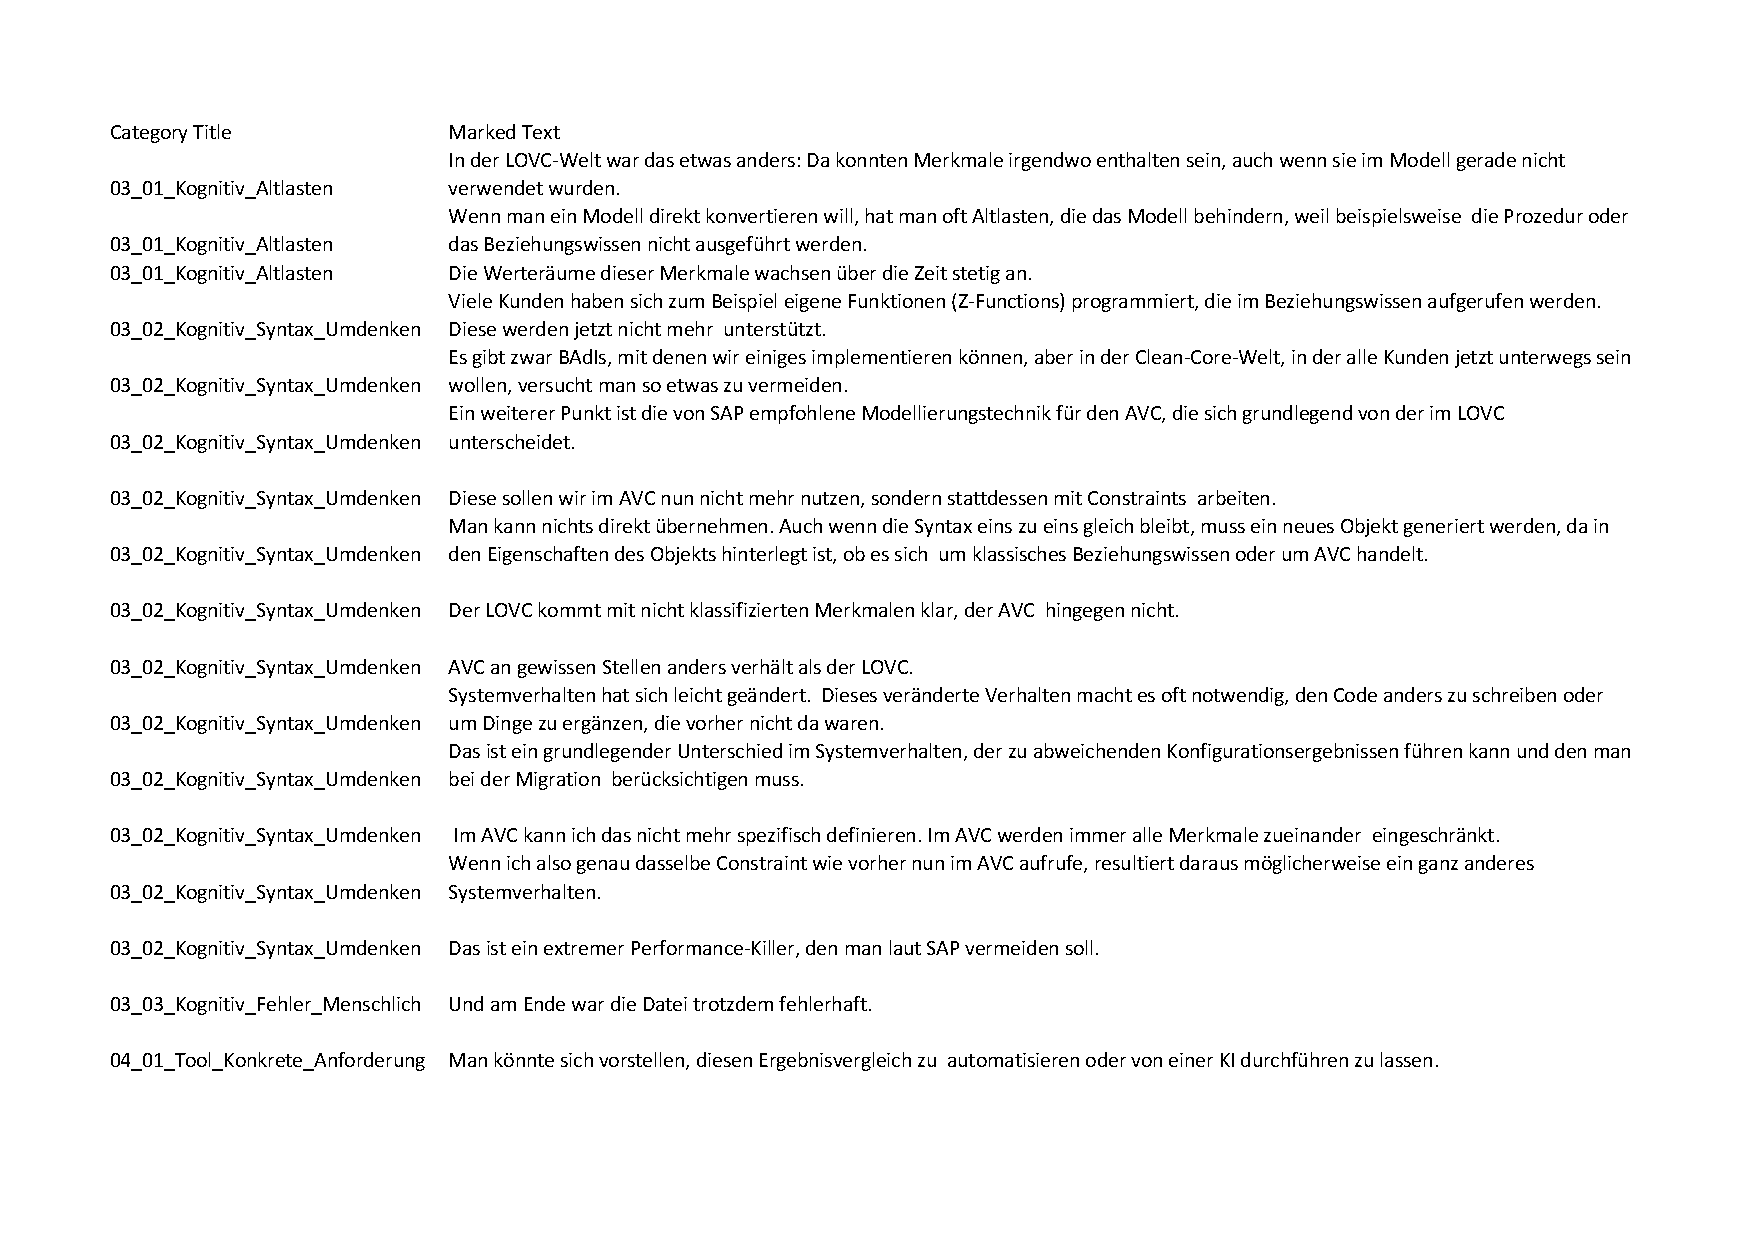
\includepdf[pages=-, scale=0.8, pagecommand={\thispagestyle{plain}}]{anhang/Codierte_Passagen_Sortiert_zusammengeführt.pdf}

\end{appendices}

\end{document}